% Course report (PLAN Phase 6, item 2). python -m ecgaug.paper writes everything this file inputs into report/generated/:
% tables, number macros, results sentences and the report's own texts (generated/report_*.tex, src/ecgaug/report_text.py),
% and every table again as Markdown in report/results.md. Never type a result by hand; a red [bracket] is a result that does
% not exist yet. Build: cd report && tectonic report.tex (figures come from ../figures/).
\documentclass[11pt]{article}
\usepackage[margin=2.5cm]{geometry}
\usepackage{microtype}
\usepackage{booktabs}
\usepackage{array}
\usepackage{longtable}
\usepackage{tocloft}\setlength{\cftbeforesecskip}{2pt}
\newcolumntype{L}[1]{>{\raggedright\arraybackslash}p{#1}}
\usepackage{graphicx}
\usepackage{adjustbox}
\usepackage{amsmath}
\usepackage{xcolor}
\usepackage{hyperref}
\hypersetup{hidelinks}
\graphicspath{{../figures/}}
\usepackage[section]{placeins}  % a section's floats are placed before the next section starts
\renewcommand{\topfraction}{0.9}\renewcommand{\bottomfraction}{0.8}\renewcommand{\textfraction}{0.07}
\renewcommand{\floatpagefraction}{0.75}\setcounter{topnumber}{3}\setcounter{totalnumber}{5}
\newcommand{\missing}[1]{\textcolor{red}{[#1]}}
% Generated by python -m ecgaug.paper; do not edit. Every value comes from a result file.
\newcommand{\CountTestF}{388}
\newcommand{\CountTestN}{44,259}
\newcommand{\CountTestS}{1,837}
\newcommand{\CountTestV}{3,221}
\newcommand{\CountTrainingF}{388}
\newcommand{\CountTrainingN}{35,496}
\newcommand{\CountTrainingS}{644}
\newcommand{\CountTrainingV}{3,030}
\newcommand{\CountValidationF}{27}
\newcommand{\CountValidationN}{10,370}
\newcommand{\CountValidationS}{300}
\newcommand{\CountValidationV}{758}
\newcommand{\PhaseOneInputRepresentationAMean}{0.164}
\newcommand{\PhaseOneInputRepresentationBMean}{0.001}
\newcommand{\PhaseOneInputRepresentationCMean}{0.296}
\newcommand{\PhaseOneInputRepresentationDMean}{0.035}
\newcommand{\PhaseTwoBaselineClassifiersAMean}{0.349}
\newcommand{\PhaseTwoBaselineClassifiersBMean}{0.231}
\newcommand{\PhaseTwoBaselineClassifiersCMean}{0.315}
\newcommand{\PhaseTwoBaselineClassifiersDMean}{0.252}
\newcommand{\PhaseOneWinner}{C}
% Written by ecgaug.final_eval; do not edit.
\newcommand{\TestCnnNoneRare}{0.088}
\newcommand{\TestCnnNoneRareLow}{0.037}
\newcommand{\TestCnnNoneRareHigh}{0.194}
\newcommand{\TestCnnClassWeightedRare}{0.113}
\newcommand{\TestCnnClassWeightedRareLow}{0.057}
\newcommand{\TestCnnClassWeightedRareHigh}{0.207}
\newcommand{\TestCnnRandomOversamplingRare}{0.136}
\newcommand{\TestCnnRandomOversamplingRareLow}{0.061}
\newcommand{\TestCnnRandomOversamplingRareHigh}{0.247}
\newcommand{\TestCnnSmoteRare}{0.070}
\newcommand{\TestCnnSmoteRareLow}{0.025}
\newcommand{\TestCnnSmoteRareHigh}{0.172}
\newcommand{\TestCnnCvaeRare}{0.113}
\newcommand{\TestCnnCvaeRareLow}{0.049}
\newcommand{\TestCnnCvaeRareHigh}{0.217}
\newcommand{\TestCnnWganGpRare}{0.079}
\newcommand{\TestCnnWganGpRareLow}{0.033}
\newcommand{\TestCnnWganGpRareHigh}{0.164}
\newcommand{\TestRnnNoneRare}{0.075}
\newcommand{\TestRnnNoneRareLow}{0.014}
\newcommand{\TestRnnNoneRareHigh}{0.232}
\newcommand{\TestRnnClassWeightedRare}{0.061}
\newcommand{\TestRnnClassWeightedRareLow}{0.022}
\newcommand{\TestRnnClassWeightedRareHigh}{0.168}
\newcommand{\TestRnnRandomOversamplingRare}{0.090}
\newcommand{\TestRnnRandomOversamplingRareLow}{0.028}
\newcommand{\TestRnnRandomOversamplingRareHigh}{0.196}
\newcommand{\TestRnnSmoteRare}{0.086}
\newcommand{\TestRnnSmoteRareLow}{0.025}
\newcommand{\TestRnnSmoteRareHigh}{0.206}
\newcommand{\TestRnnCvaeRare}{0.073}
\newcommand{\TestRnnCvaeRareLow}{0.035}
\newcommand{\TestRnnCvaeRareHigh}{0.157}
\newcommand{\TestRnnWganGpRare}{0.069}
\newcommand{\TestRnnWganGpRareLow}{0.027}
\newcommand{\TestRnnWganGpRareHigh}{0.156}
\newcommand{\TestCnnCvaeVsNoneDiff}{0.025}
\newcommand{\TestCnnCvaeVsNoneLow}{-0.018}
\newcommand{\TestCnnCvaeVsNoneHigh}{0.047}
\newcommand{\TestCnnCvaeVsNonePHolm}{1.0000}
\newcommand{\TestCnnWganGpVsNoneDiff}{-0.009}
\newcommand{\TestCnnWganGpVsNoneLow}{-0.045}
\newcommand{\TestCnnWganGpVsNoneHigh}{0.015}
\newcommand{\TestCnnWganGpVsNonePHolm}{1.0000}
\newcommand{\TestRnnCvaeVsNoneDiff}{-0.002}
\newcommand{\TestRnnCvaeVsNoneLow}{-0.100}
\newcommand{\TestRnnCvaeVsNoneHigh}{0.032}
\newcommand{\TestRnnCvaeVsNonePHolm}{1.0000}
\newcommand{\TestRnnWganGpVsNoneDiff}{-0.006}
\newcommand{\TestRnnWganGpVsNoneLow}{-0.138}
\newcommand{\TestRnnWganGpVsNoneHigh}{0.035}
\newcommand{\TestRnnWganGpVsNonePHolm}{1.0000}
\newcommand{\TestCnnCvaeVsWganGpDiff}{0.034}
\newcommand{\TestCnnCvaeVsWganGpLow}{-0.002}
\newcommand{\TestCnnCvaeVsWganGpHigh}{0.068}
\newcommand{\TestCnnCvaeVsWganGpPHolm}{0.5504}
\newcommand{\TestCnnCvaeVsSmoteDiff}{0.044}
\newcommand{\TestCnnCvaeVsSmoteLow}{-0.029}
\newcommand{\TestCnnCvaeVsSmoteHigh}{0.072}
\newcommand{\TestCnnCvaeVsSmotePHolm}{1.0000}
\newcommand{\TestCnnCvaeVsClassWeightedDiff}{0.001}
\newcommand{\TestCnnCvaeVsClassWeightedLow}{-0.041}
\newcommand{\TestCnnCvaeVsClassWeightedHigh}{0.042}
\newcommand{\TestCnnCvaeVsClassWeightedPHolm}{1.0000}
\newcommand{\TestCnnCvaeVsRandomOversamplingDiff}{-0.022}
\newcommand{\TestCnnCvaeVsRandomOversamplingLow}{-0.074}
\newcommand{\TestCnnCvaeVsRandomOversamplingHigh}{0.010}
\newcommand{\TestCnnCvaeVsRandomOversamplingPHolm}{1.0000}
\newcommand{\TestRnnCvaeVsWganGpDiff}{0.004}
\newcommand{\TestRnnCvaeVsWganGpLow}{-0.027}
\newcommand{\TestRnnCvaeVsWganGpHigh}{0.065}
\newcommand{\TestRnnCvaeVsWganGpPHolm}{1.0000}
\newcommand{\TestRnnCvaeVsSmoteDiff}{-0.013}
\newcommand{\TestRnnCvaeVsSmoteLow}{-0.067}
\newcommand{\TestRnnCvaeVsSmoteHigh}{0.016}
\newcommand{\TestRnnCvaeVsSmotePHolm}{1.0000}
\newcommand{\TestRnnCvaeVsClassWeightedDiff}{0.012}
\newcommand{\TestRnnCvaeVsClassWeightedLow}{-0.047}
\newcommand{\TestRnnCvaeVsClassWeightedHigh}{0.039}
\newcommand{\TestRnnCvaeVsClassWeightedPHolm}{1.0000}
\newcommand{\TestRnnCvaeVsRandomOversamplingDiff}{-0.016}
\newcommand{\TestRnnCvaeVsRandomOversamplingLow}{-0.059}
\newcommand{\TestRnnCvaeVsRandomOversamplingHigh}{0.016}
\newcommand{\TestRnnCvaeVsRandomOversamplingPHolm}{1.0000}



\title{Rare-Arrhythmia Detection with Generative ECG Augmentation\\\large Course project report}
\author{\missing{team members}}
\date{}

\begin{document}
\maketitle

\begin{abstract}
We built a system that takes one ECG beat and returns its class, normal (N), supraventricular ectopic (S), ventricular ectopic (V) or fusion (F), a saliency map of the parts of the beat behind the prediction, and a short note for a clinician that is checked against the model output. With it we asked whether synthetic beats of the rare classes from a conditional VAE or a WGAN-GP help a model find them in patients it has never seen. Every choice was fixed on validation patients by rules written down in advance, and the 22 test patients of the MIT-BIH Arrhythmia Database were read once. Generative augmentation was detectably better than no augmentation in 0 of 4 pre-registered comparisons, and the best pre-registered model reached a rare-class macro-F1 (the mean of S and F F1) of 0.136. The cnn without augmentation, 0.088 on new patients, scored 0.777 to 0.837 with the same patients in training and test. Follow-up analyses, each registered before it ran, found what moves the score: each beat seen relative to the patient's own normal beat (0.088 to 0.371), prematurity judged against the recording's mean heart period, no S calls during atrial fibrillation, and ten runs averaged; together they reached 0.587 on the test records, close to the best published inter-patient result we could check (0.582). That score is optimistic after repeated reads of the test records: on 977 unused patients the pipeline's S F1 was 0.294, against 0.647 on the test records. Patient variation, not class rarity, limits these models; more training patients with rare beats, larger models and more runs are needed to establish how much augmentation can add.

\end{abstract}

\setcounter{tocdepth}{1}
\tableofcontents

\section{Introduction}
Most heartbeats are normal, and the beats that matter clinically are rare. A day-long ECG recording holds about a hundred thousand
beats, of which usually only a small share come too early from the atria or the ventricles; software has to find those so that a
clinician can review them. Machine-learning models learn the common normal beat well and the rare classes poorly, and a popular remedy is to
train them on synthetic examples of the rare classes made by a generative model.

This project builds a complete system and uses it to test that remedy honestly. The system takes one ECG beat and returns a
predicted class, a saliency map showing which parts of the beat drove the prediction, and a short note for a clinician that is
checked against the model output. The research question is whether class-conditional generative augmentation, with a conditional
VAE~\cite{sohn2015cvae} or a WGAN-GP~\cite{gulrajani2017wgangp}, improves detection of the rare classes S and F compared with no
augmentation, class-weighted loss, random oversampling and SMOTE~\cite{chawla2002smote}, when the model is tested on patients it has
never seen~\cite{dechazal2004}. The project delivers:
\begin{itemize}
\item \textbf{A working system} from beat to class, saliency map and checked note, with a command that runs it end to end.
\item \textbf{A controlled comparison} of the two generators against no augmentation and three simpler rebalancing methods, with two
classifiers, several seeds, uncertainty over patients and selection rules written down before each experiment.
\item \textbf{Three side questions}: how much testing on patients seen in training inflates the score, whether metrics of synthetic-beat
quality predict the benefit, and whether augmentation changes what the classifier looks at.
\item \textbf{Follow-up analyses} of why augmentation did not help and what did, ending in a pipeline checked on patients that no
analysis had used.
\end{itemize}

Section~\ref{sec:medical} explains the medical background: what the beat classes are, why they matter and why new patients make
them hard. Section~\ref{sec:related} places the project among earlier work, Section~\ref{sec:protocol} gives the data and the evaluation
rules, Section~\ref{sec:system} the system and every model tested, and Section~\ref{sec:development} how each part was chosen.
Section~\ref{sec:results} gives the pre-registered results, Section~\ref{sec:posthoc} the follow-up analyses and
Section~\ref{sec:all-results} every metric beside published results; Sections~\ref{sec:discussion} to~\ref{sec:reproducibility} discuss
them and say what limits them.

\section{Medical background}\label{sec:medical}

\paragraph{The heartbeat and the ECG.} Each heartbeat starts in the sinoatrial node, a small group of pacemaker cells in the right
atrium. The impulse spreads across both atria, which contract; on the ECG this is the P wave. It is then delayed in the
atrioventricular (AV) node, which gives the atria time to empty into the ventricles, runs down the His bundle and the left and right
bundle branches, and spreads through both ventricles within a few hundredths of a second: the QRS complex, normally narrower than
120~ms. The recovery of the ventricles (repolarisation) is the T wave. The time between two consecutive beats, measured between their
R peaks, is the RR interval; a normal resting (sinus) rhythm of 60 to 100 beats per minute has RR intervals of 0.6 to
1~s~\cite{goldberger2017}. Figure~\ref{fig:medical} shows these waves on real recordings.

\paragraph{The beat classes.} The AAMI standard for testing arrhythmia algorithms~\cite{aami2012ec57} groups the beat labels of the
annotators into five classes (Table~\ref{tab:classes}). The first four are used here; Q holds paced and unclassifiable beats and is
excluded, as are the four records of patients with pacemakers.

\begin{table}[tbp]\centering\footnotesize\setlength{\tabcolsep}{4pt}
\caption{The AAMI beat classes, the MIT-BIH labels in each, and what they mean clinically~\cite{goldberger2017,aami2012ec57}.}\label{tab:classes}
\begin{tabular}{@{}L{0.2\linewidth}L{0.2\linewidth}L{0.28\linewidth}L{0.26\linewidth}@{}}
\toprule
Class (MIT-BIH labels) & Where it starts & How it looks on the ECG & Why it matters \\
\midrule
\textbf{N}, normal (normal; left and right bundle branch block; atrial and junctional escape) & the sinus node, through the normal
conduction path (in bundle branch block one branch conducts late) & a P wave before every QRS and a regular rhythm; the QRS is narrow, or
wide in bundle branch block & the reference every other beat is judged against \\ \addlinespace
\textbf{S}, supraventricular ectopic (atrial, aberrated atrial, junctional and supraventricular premature beats) & an early impulse in
the atria or the AV junction, outside the sinus node & comes early (a short RR interval before it); the QRS is usually like the patient's
normal one; the P wave is different or hidden & frequent S beats go with later atrial fibrillation and stroke~\cite{binici2010}; runs
of them are supraventricular tachycardia \\ \addlinespace
\textbf{V}, ventricular ectopic (premature ventricular contractions; ventricular escape beats) & an impulse in the ventricle muscle,
spreading cell to cell rather than through the conduction system & comes early; a wide, bizarre QRS (120~ms or more) with no P wave
before it and a T wave pointing the other way; usually a full pause after it & a high burden of V beats goes with a weakened left
ventricle~\cite{baman2010}; three or more in a row are ventricular tachycardia, which can be life-threatening \\ \addlinespace
\textbf{F}, fusion (fusion of a ventricular and a normal beat) & a ventricular and a normal impulse that activate the ventricles at the
same moment & a QRS whose shape lies between the patient's normal and ventricular beats & harmless in itself, but a sign of ventricular
ectopic activity; rare and different in every patient \\ \addlinespace
\textbf{Q}, other (paced; fusion of paced and normal; unclassifiable) & a pacemaker, or unknown & --- & excluded here \\
\bottomrule
\end{tabular}
\end{table}

\paragraph{How the beats are used in the clinic.} An ambulatory (Holter) monitor records the ECG for one or more days while the
patient goes about daily life~\cite{steinberg2017}; at 70 beats per minute a day holds about 100,000 beats. No one reads them one by
one: software detects and classifies every beat, counts the ectopic beats and flags runs and pauses, and a technician or cardiologist
reviews what it flags. The software must therefore find the rare beats (high sensitivity) without burying the reader in false alarms
(high positive predictivity, the share of its calls that are right). The AAMI standard asks for both, for every
class~\cite{aami2012ec57}; this report gives both and their harmonic mean, the F1 score.

\paragraph{Why new patients are hard.} Every patient's ECG looks different: the position and axis of the heart, the build of the
body, where the electrodes sit and any disease of the conduction system all change the shape of the same kind of beat. A patient with
bundle branch block has normal beats as wide as another patient's V beats, and an S beat in one patient can look exactly like a normal
beat in another (Figure~\ref{fig:medical}C). What identifies an S beat is mostly its timing: it comes earlier than this patient's own
rhythm predicts. Cardiologists therefore judge prematurity against the patient's underlying rhythm, and they do not call S beats during
atrial fibrillation, where the atria quiver without organised activity, there are no P waves and the ventricular rhythm is irregular,
so early beats are expected. A model tested on beats of patients it has seen can recognise the patient instead of the arrhythmia; a
model tested on new patients has to learn these patient-relative cues. Software meets a new patient every time it is used, so this
project trains and tests on different patients, the inter-patient protocol of de Chazal et al.~\cite{dechazal2004}. Several of the
follow-up analyses (Section~\ref{sec:posthoc}) build exactly these clinical cues into the system.

\paragraph{The database.} The MIT-BIH Arrhythmia Database~\cite{moody2001,goldberger2000} holds 48 half-hour excerpts of two-lead
Holter recordings from 47 patients of Boston's Beth Israel Hospital, recorded between 1975 and 1979 and digitised at 360 samples per
second. Twenty-three recordings were chosen at random and 25 to include less common but clinically important arrhythmias, so the rare
classes sit in a few patients each; two or more cardiologists labelled every beat independently and resolved their disagreements. This
project uses lead MLII, a modified limb lead with the electrodes on the chest.

\begin{figure}[htbp]\centering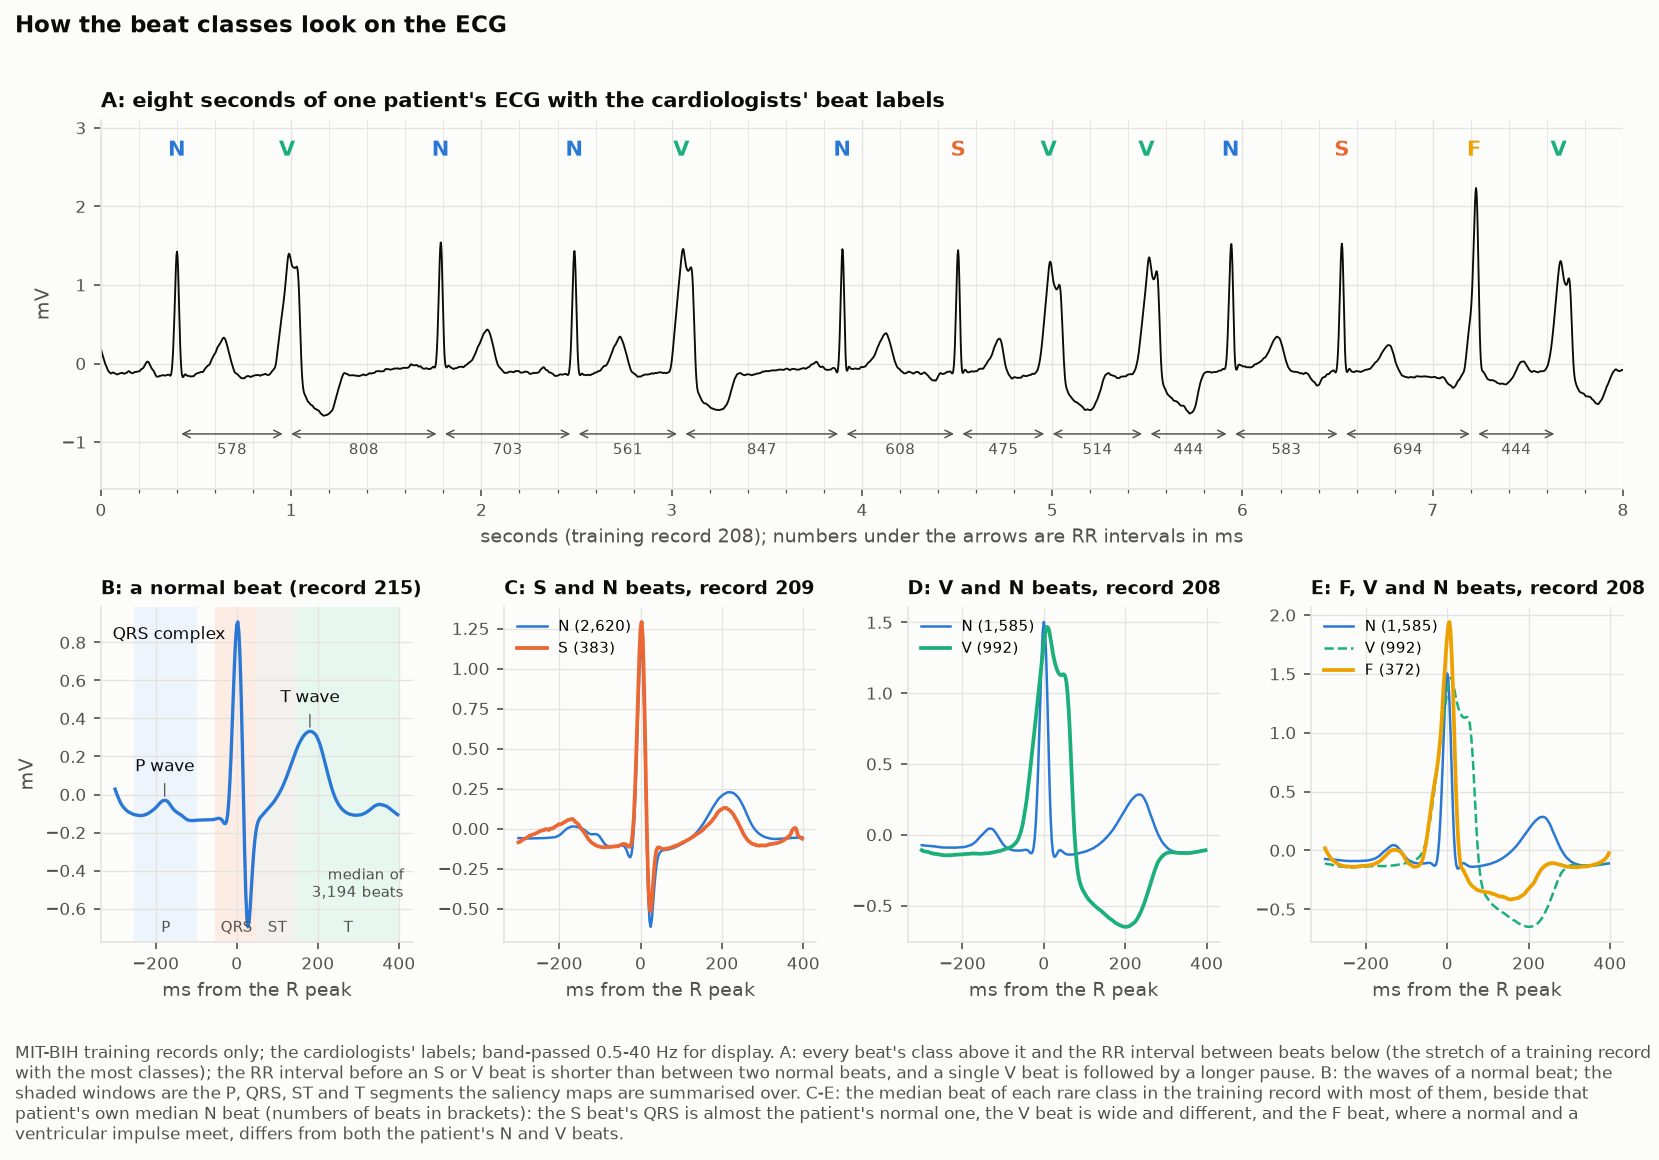
\includegraphics[width=\linewidth]{report/medical_background.png}
\caption{The beat classes on real MIT-BIH training recordings. A: eight seconds of one patient with the cardiologists' labels and the
RR intervals; the S and V beats come early. B: the waves of a normal beat and the four windows over which the saliency maps are
summarised. C--E: the median S, V and F beats of the training patients with most of each, beside the same patient's normal beats.}
\label{fig:medical}\end{figure}

\paragraph{What this system is not.} It is a course project and not a medical device. It has not been validated clinically, and its
notes are machine-written summaries of the model output for a clinician to check, never a diagnosis.

\section{Related work}\label{sec:related}
\paragraph{Evaluation protocols.} The AAMI EC57 standard~\cite{aami2012ec57} groups MIT-BIH beat labels into the classes N, S, V, F
and Q and asks for record-by-record reporting. De Chazal et al.~\cite{dechazal2004} introduced the DS1/DS2 inter-patient split used
here; Llamedo and Mart\'inez~\cite{llamedo2011} selected features by how well they generalise across databases, and a recent
systematic review finds that only a minority of studies follow these standards~\cite{silva2025review}. Many studies split beats at
random, so beats of the same patient appear in training and test; their scores are much higher than inter-patient
ones~\cite{mousavi2019}, and Section~\ref{sec:results} measures that gap for this pipeline.

\paragraph{Inter-patient classifiers.} The strongest inter-patient results lean on RR intervals normalised to the patient's own rhythm:
Lin and Yang~\cite{lin2014} normalise RR intervals by the recording's mean, Huang et al.~\cite{huang2014} add a stage that calls a beat
S when it comes early against that mean, Mond\'ejar-Guerra et al.~\cite{mondejar2019} and Saenz-Cogollo and Agelli~\cite{saenz2020}
combine RR and shape features in ensembles and random forests, and Zhu et al.~\cite{zhu2022} feed RR intervals to a convolutional network.
Section~\ref{sec:all-results} compares this project with them, and several follow-up analyses test their ideas here.

\paragraph{Generative augmentation of ECG.} Recurrent conditional GANs were proposed for medical time series and evaluated by training
on synthetic and testing on real data~\cite{esteban2017rcgan}. GANs have been used to synthesise realistic ECG~\cite{delaney2019ecggan}
and to augment MIT-BIH classifiers~\cite{shaker2020gan}; an auxiliary-classifier WGAN-GP with DTW-based screening is closest to the
WGAN-GP variants here~\cite{adib2022cgan}. SimGANs~\cite{golany2020simgans} add McSharry et al.'s ECG simulator~\cite{mcsharry2003dynamical}
to the generator's loss, and conditional diffusion models now generate ECG~\cite{alcaraz2023sssd} and have been used to augment beat classifiers~\cite{kwak2024diffusion};
both are tested as follow-ups. The generators build on the VAE~\cite{kingma2013vae}, its conditional form~\cite{sohn2015cvae}, the
Wasserstein GAN~\cite{arjovsky2017wgan} with gradient penalty~\cite{gulrajani2017wgangp}, and the conditioning schemes of auxiliary
classifiers~\cite{odena2016acgan}, projection critics~\cite{miyato2018projection} and FiLM~\cite{perez2018film}.

\paragraph{Synthetic-quality metrics, explanations and reports.} Synthetic beats are scored with dynamic time
warping~\cite{sakoe1978dtw}, spectral distances, a Fr\'echet distance in the feature space of a fixed network after
FID~\cite{heusel2017fid}, train-on-synthetic-test-on-real~\cite{esteban2017rcgan} and classifier two-sample
tests~\cite{lopezpaz2017c2st}. The saliency methods compared are Grad-CAM~\cite{selvaraju2016gradcam}, integrated
gradients~\cite{sundararajan2017ig}, SmoothGrad~\cite{smilkov2017smoothgrad} and occlusion. Large ECG-language models can write
diagnostic reports~\cite{zhao2024ecgchat}; the note generator here instead restates the classifier output and is checked claim by claim.

\section{Data and evaluation protocol}\label{sec:protocol}
The records are split by patient as de Chazal et al.\ proposed~\cite{dechazal2004}: the 22 DS1 records give training and validation
and the 22 DS2 records the test set, so no patient is in two splits (Table~\ref{tab:data}). The validation set is a patient-wise subset
of DS1 (records 115, 118, 201, 205 and 223), chosen from DS1 class counts only and fixed at the first gate. One subject appears as
record 201 in DS1 and record 202 in DS2; the split is kept for comparability, and the test results are also reported without record 202.

\paragraph{Beats.} Lead MLII is selected by its name in each record's header, never by channel position. The reference annotations are
mapped to the AAMI classes, RR intervals are measured between consecutive QRS annotations before any class is dropped, and the few Q beats
are left out of training and metrics. A beat is usable when its window fits in the record and both neighbouring RR intervals exist; the
same rule holds for every input representation, so the set of beats never depends on the representation. Each beat is a window around
its annotated R peak, z-scored, with its RR intervals as side input (representation \PhaseOneWinner, chosen on validation;
Section~\ref{sec:development}).

\begin{table}[htbp]\centering\small% Generated by python -m ecgaug.paper from: results/phase1_data/record_counts.csv
\begin{tabular}{lrrrrr}
\toprule
Split & Records & N & S & V & F \\
\midrule
training & 17 & 35,496 & 644 & 3,030 & 388 \\
validation & 5 & 10,370 & 300 & 758 & 27 \\
test (DS2) & 22 & 44,259 & 1,837 & 3,221 & 388 \\
\bottomrule
\end{tabular}
\caption{Records and beats per split.}\label{tab:data}\end{table}

\paragraph{Metrics.} For each class, sensitivity is the share of its beats that the model finds and positive predictivity the share
of the model's calls of that class that are right; F1 is their harmonic mean. The primary metric is the rare-class macro-F1, the mean of
the S and F F1 scores on the test records. The validation records hold fewer F beats than the minimum fixed in advance, so model choices
use validation S F1 with V F1 as tie-break; the test metric is unchanged. Decisions are the most probable class; no threshold is tuned.
Secondary metrics are per-class F1, one-vs-rest PR-AUC, sensitivity and positive predictivity for S and V, normal recall and the
macro-F1 over all four classes.

\paragraph{Statistics.} Beats of one patient are correlated, so uncertainty comes from resampling the 22 test records (a cluster
bootstrap with 10,000 resamples; seeds averaged within each resample). Paired differences resample the same records for both conditions,
and two-sided bootstrap $p$-values are adjusted with Holm's method~\cite{holm1979} within two families: the four confirmatory
comparisons (each generator against no augmentation, for each of the two classifiers) and eight secondary ones (cVAE against WGAN-GP, and
the best generative condition against each rebalancing method). Resamples in which S or F has no true beats are left out and counted.

\paragraph{Rules fixed in advance.} The project ran in five phases with a human-approved gate after each. At every phase four variants
were compared on validation: four input representations, four classifiers, four families of synthetic-quality metrics, four cVAE and
four WGAN-GP designs, four augmentation policies, four saliency methods and four note generators, each chosen by a rule written in the
pre-registration before the comparison ran. The final grid trains six conditions at three strengths for two classifiers and three
seeds. The test records sit in a separate file that only a guarded loader can read; every read is logged, and the pre-registered test
was read once, after every choice had been fixed.

\section{The system and its architecture}\label{sec:system}
\begin{enumerate}
\item \textbf{Beat extraction}: a window around the reference R peak (representation \PhaseOneWinner), z-scored per beat, with the RR
features as side input.
\item \textbf{Classifier}: the cnn chosen at the phase 2 gate, trained with the augmentation condition chosen on validation.
\item \textbf{Saliency}: the method chosen per classifier at the phase 5 gate (Grad-CAM~\cite{selvaraju2016gradcam} for the cnn,
occlusion for the rnn), summarised as the share of saliency in the P, QRS, ST and T windows around the R peak
(Figure~\ref{fig:medical}B).
\item \textbf{Note}: a generator writes a note from a JSON object holding only the prediction, the probabilities, a low-confidence flag
and the two segments with the most saliency; a fact checker rejects any claim not in that object, and a template note replaces any note
that fails the check (Figure~\ref{fig:example}).
\end{enumerate}
The command \texttt{python -m ecgaug.demo --record <validation record> --beat <index>} runs it end to end; it prints the prediction,
the probabilities and the note, and saves a figure of the beat with its saliency.

\begin{figure}[p]\centering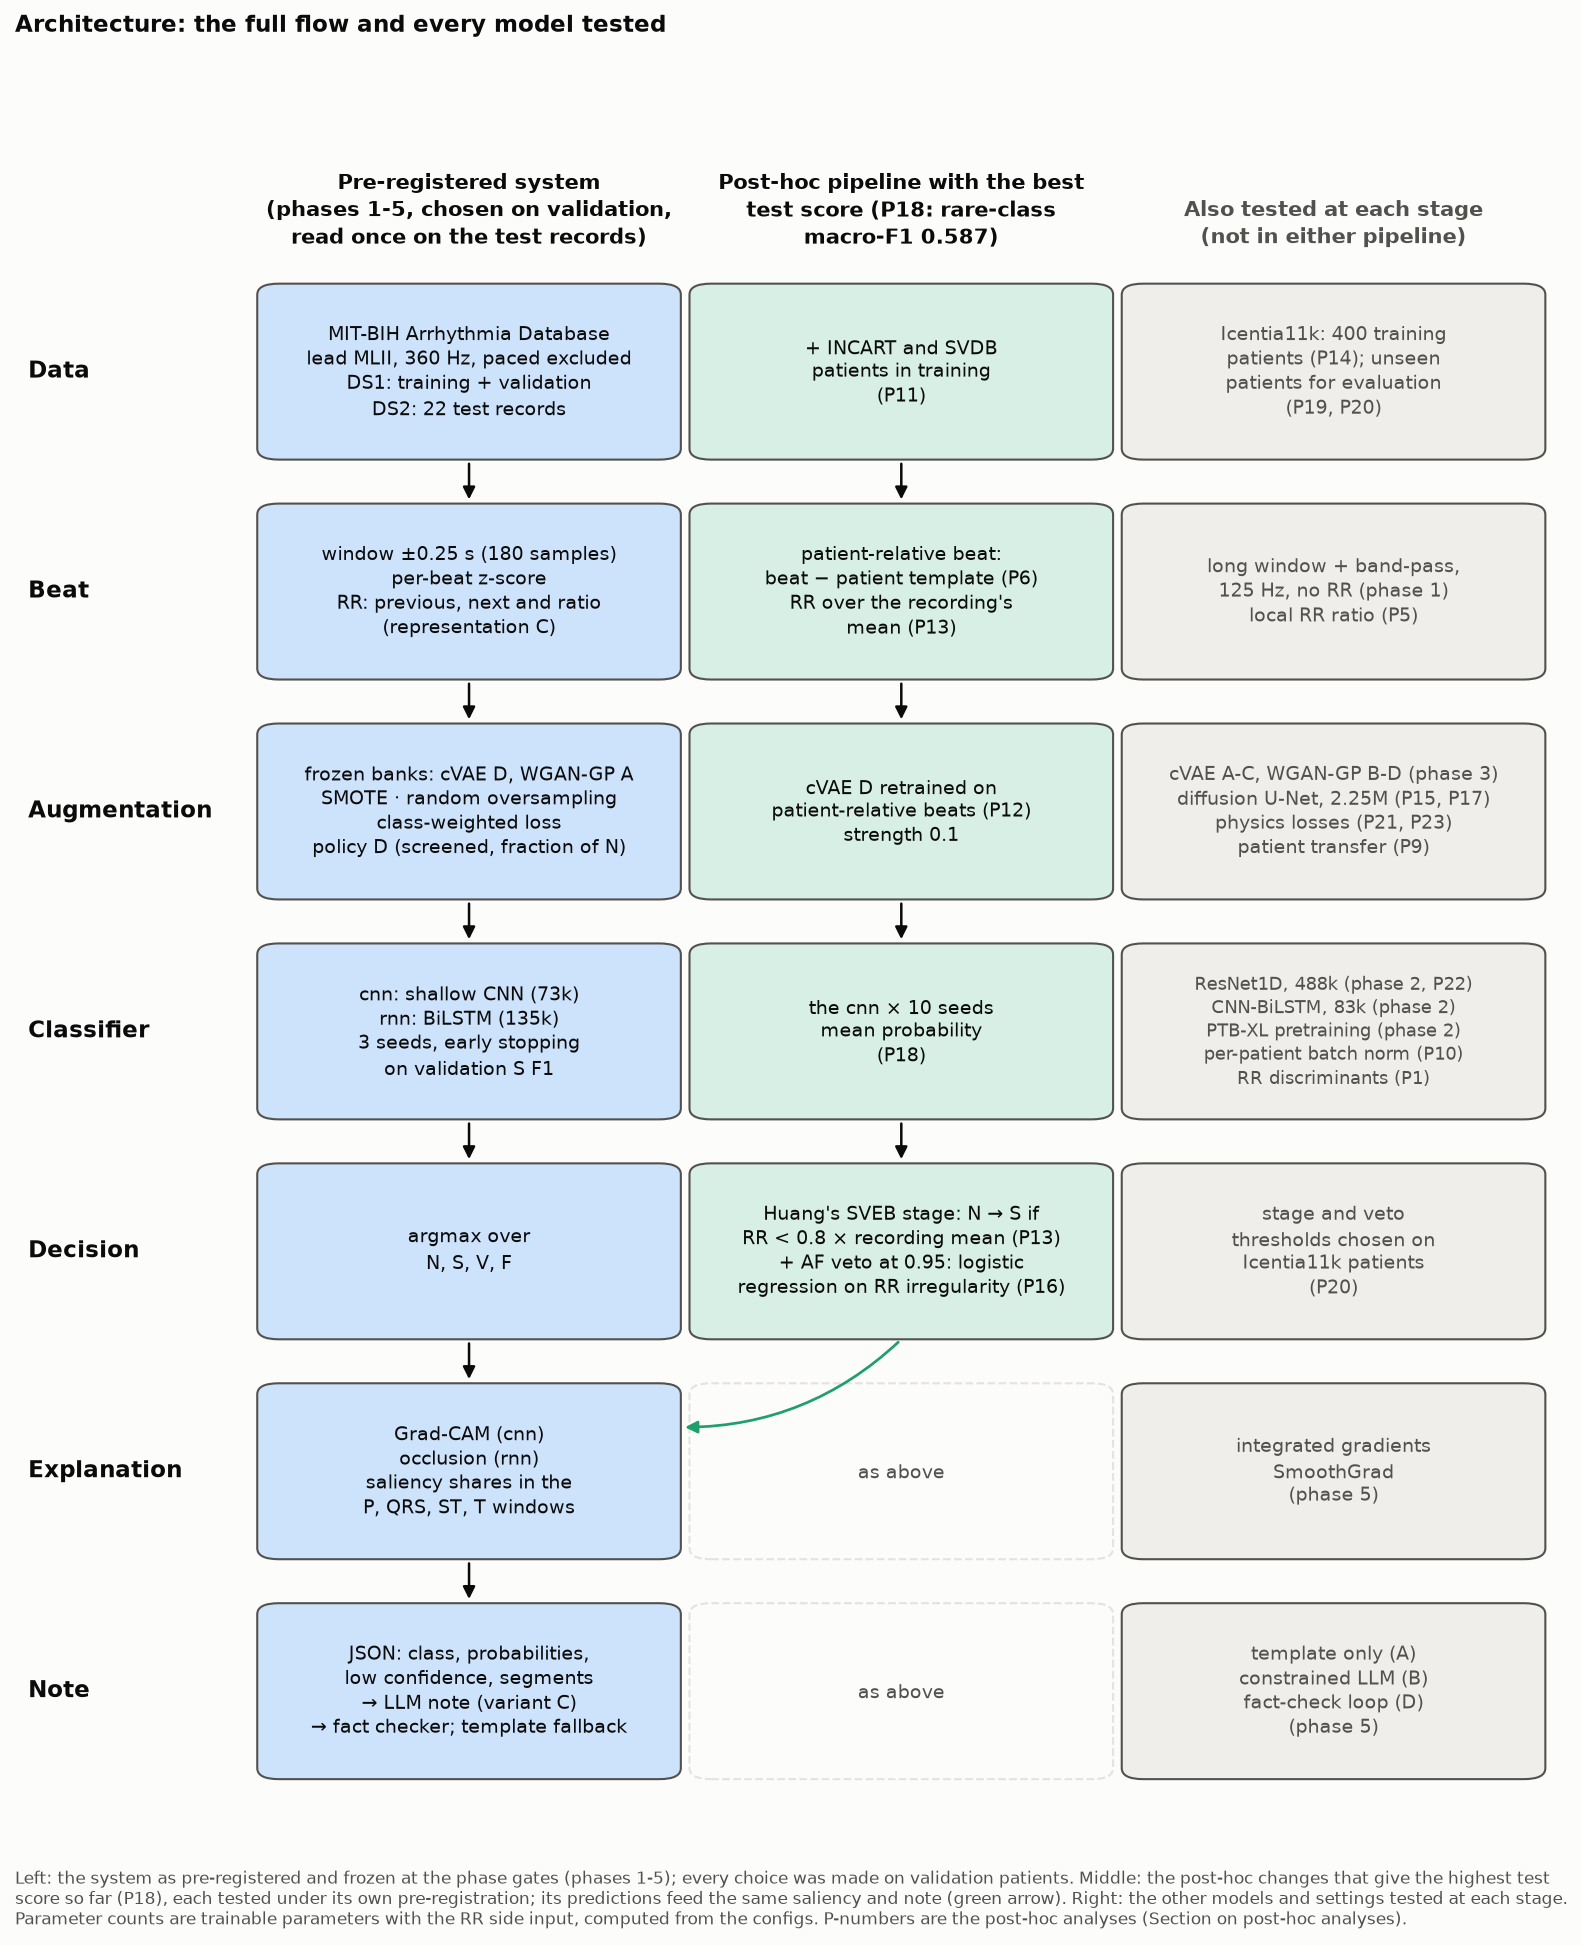
\includegraphics[width=0.92\linewidth]{architecture/flow.png}\caption{The full flow: the pre-registered
system (left), the post-hoc pipeline with the best test score (middle) and what else was tested at each stage (right).}
\label{fig:architecture}\end{figure}

\begin{figure}[htbp]\centering
\fbox{\begin{minipage}[t]{0.46\linewidth}\footnotesize
\textbf{Input} (validation beat labelled S by the cardiologists)\par\smallskip
\begin{tabular}{@{}p{0.3\linewidth}p{0.64\linewidth}@{}}
predicted class & S \\
probabilities & N 0.00, S 0.93, V 0.06, F 0.00 \\
low confidence & no \\
saliency share & P 0.55, ST 0.26
\end{tabular}\par\medskip
\textbf{Note} (generator C; 0 unsupported claims)\par\smallskip
\emph{The beat is classified as a supraventricular ectopic beat (S) with a probability of 0.93. The top segments are the P wave with a mass of 0.55 and the ST segment with a mass of 0.26. This note was generated automatically by a research model. It is not a diagnosis and must be reviewed by a clinician.}
\end{minipage}}\hfill
\fbox{\begin{minipage}[t]{0.46\linewidth}\footnotesize
\textbf{Input} (validation beat labelled V by the cardiologists)\par\smallskip
\begin{tabular}{@{}p{0.3\linewidth}p{0.64\linewidth}@{}}
predicted class & V \\
probabilities & N 0.04, S 0.00, V 0.95, F 0.01 \\
low confidence & no \\
saliency share & QRS 0.63, ST 0.35
\end{tabular}\par\medskip
\textbf{Note} (generator C; 0 unsupported claims)\par\smallskip
\emph{The heartbeat classifier predicts the beat is a ventricular ectopic beat (V) with a probability of 0.95. The top segments contributing to this prediction are the QRS complex with a mass of 0.63 and the ST segment with a mass of 0.35. This note was generated automatically by a research model. It is not a diagnosis and must be reviewed by a clinician.}
\end{minipage}}
\caption{The system's output for two validation beats, the first S and the first V beat of the note cases that the model classified correctly with confidence. The note generator receives only the input object, never the signal; the fact checker compares every claim of the note with it, and a template note replaces any note that fails. Saliency shares are the fractions of the saliency map inside the P, QRS, ST and T windows of Figure~\ref{fig:medical}; the two largest are passed on.}\label{fig:example}
\end{figure}


Figure~\ref{fig:architecture} shows the whole system as one flow. The top row is the system as pre-registered and frozen at the phase gates: a beat window from lead MLII with its RR features, an optional synthetic bank, a classifier, argmax, a saliency map and a note checked against the model output. The middle row is the post-hoc pipeline with the highest test score so far (P18), and the bottom row lists what else was tried at each stage. Tables~\ref{tab:arch-classifiers} to~\ref{tab:arch-other} list every model that was trained or tested, 30 entries in all, 15 of them neural networks with their trainable parameters counted from their configurations (with the three RR side features where the model takes them). Every choice among them was made on validation patients by a rule written down before the comparison.
\begingroup\footnotesize
\begin{longtable}{p{2.6cm}p{6.1cm}rp{4.6cm}}
\caption{Classifiers and other models fitted to beats. Bold: chosen by a pre-registered rule.}\label{tab:arch-classifiers}\\
\toprule
Model & Structure & Parameters & Where it ran; outcome \\
\midrule
\endfirsthead
\toprule
Model & Structure & Parameters & Where it ran; outcome \\
\midrule
\endhead
\bottomrule
\endfoot
Probe CNN & 3 conv blocks (16, 32, 64 channels, kernel 7), global average pooling, RR side branch, linear head & 18,762 & phase 1 (input choice); quality metrics (TSTR, feature network); a measuring instrument, not a candidate \\
\textbf{Shallow CNN (the cnn)} & 3 conv-BN-ReLU-max-pool blocks (32, 64, 128, kernel 7), global average pooling; RR side branch (batch norm, 16 units); linear head & 73,226 & phase 2 variant A; every later experiment; validation S F1 0.349 (SD 0.045) at phase 2; chosen as the cnn \\
ResNet1D & stem conv, 4 residual stages (32, 64, 128, 128, kernel 7, two conv-BN each with a shortcut), global average pooling, RR side branch, linear head & 488,362 & phase 2 variant B; P22; validation S F1 0.231 (SD 0.097) at phase 2; not chosen; re-tested in P18's pipeline as P22: against the cnn, S F1 on P19's patients no augmentation +0.021, cVAE +0.023 (detectable), WGAN-GP +0.058 (detectable); test rare-class macro-F1 no augmentation +0.056, cVAE +0.027, WGAN-GP $-$0.246 \\
\textbf{BiLSTM (the rnn)} & 2-layer bidirectional LSTM (64 units), last states and mean output concatenated, RR side branch, linear head & 134,794 & phase 2 variant C; full grid; P5, P13; validation S F1 0.315 (SD 0.020) at phase 2; chosen as the rnn \\
CNN-BiLSTM & 2 conv blocks (32, 64, kernel 7), 1 bidirectional LSTM layer (64 units), RR side branch, linear head & 82,570 & phase 2 variant D; validation S F1 0.252 (SD 0.029) at phase 2; not chosen \\
PTB-XL pretraining & the probe CNN pretrained on PTB-XL beats with their recording's five diagnostic superclasses, then fine-tuned on MIT-BIH & 18,762 & phase 2 (two arms: RR features, 125 Hz); from-scratch training kept in both arms \\
Per-patient batch norm & frozen cnn or rnn whose batch-norm statistics are recomputed from each patient's beats & -- & P10; no new parameters; post hoc \\
RR linear discriminants & LDA on the three RR features, and on them plus every 10th sample of the beat (de Chazal-style) & -- & P1; fixed references beside the cnn; post hoc \\
Logistic regression, gradient boosting & models of the RR intervals compared with rules on training-side patients & -- & P14; descriptive check only \\
\end{longtable}
\endgroup
\begingroup\footnotesize
\begin{longtable}{p{2.6cm}p{6.1cm}rp{4.6cm}}
\caption{Generators, generator objectives and augmentation without a learned model. Bold: chosen by a pre-registered rule.}\label{tab:arch-generators}\\
\toprule
Model & Structure & Parameters & Where it ran; outcome \\
\midrule
\endfirsthead
\toprule
Model & Structure & Parameters & Where it ran; outcome \\
\midrule
\endhead
\bottomrule
\endfoot
cVAE A & conv encoder and decoder, class one-hot concatenated to the input and the latent code, latent 16, KL weight annealed over 30\% of steps & 415,905 & phase 3; pilots; not chosen at the phase 3 gate \\
cVAE B & as A with a smaller KL weight (0.1 and 0.25) & 415,905 & phase 3; pilots; not chosen at the phase 3 gate \\
cVAE C & as A plus an L1 loss between FFT magnitudes & 415,905 & phase 3; pilots; not chosen at the phase 3 gate \\
\textbf{cVAE D} & residual encoder and decoder with FiLM class conditioning in every block & 803,841 & phase 3; P12 (retrained on patient-relative beats), P21, P23; chosen at the phase 3 gate \\
\textbf{WGAN-GP A} & label embedding concatenated to the noise (64) and as a class channel to the critic; 5 critic steps, gradient penalty 10 & 501,362 & phase 3; P12 (retrained on patient-relative beats), P21, P23; chosen at the phase 3 gate \\
WGAN-GP B & projection critic & 512,194 & phase 3; pilots; not chosen at the phase 3 gate \\
WGAN-GP C & auxiliary class head on the critic (AC-WGAN-GP) & 512,198 & phase 3; pilots; not chosen at the phase 3 gate \\
WGAN-GP D & one unconditional WGAN-GP per class S, V, F & 1,359,750 & phase 3; pilots; not chosen at the phase 3 gate \\
Diffusion (1D U-Net) & 1D U-Net (64, 128, 256 channels, kernel 5), 1,000-step cosine schedule, DDIM sampling in 50 steps, classifier-free guidance 1.5, EMA weights & 2,250,497 & P15; P17 (five times longer); post hoc; one of P18's six conditions \\
Physics loss, drawn parameters & McSharry et al.'s ECG equation, Euler residual with 16 parameters drawn from the class (SimGANs) & -- & P21; barely moved the generators; post hoc \\
Physics loss, fitted heights & the simulator's best fit with the class's wave timing, heights and baseline solved per beat & -- & P23; moved the generators (large weights smooth the banks); small S gain on P19's patients for the cVAE; post hoc \\
SMOTE, random oversampling, class weights & interpolation between same-class beats; repeated real beats; class-weighted cross-entropy & -- & phase 4 grid; P5-P18; the pre-registered comparison conditions \\
Patient transfer, fusion beats & a real deviation placed on other patients' templates (P9); a fraction of a real V deviation as F (P21) & -- & P9; P21; fusion beats stopped by their pre-registered rule \\
\end{longtable}
\endgroup
\begingroup\footnotesize
\begin{longtable}{p{2.6cm}p{6.1cm}rp{4.6cm}}
\caption{Decision rules, explanation and note generation. Bold: chosen by a pre-registered rule.}\label{tab:arch-other}\\
\toprule
Model & Structure & Parameters & Where it ran; outcome \\
\midrule
\endfirsthead
\toprule
Model & Structure & Parameters & Where it ran; outcome \\
\midrule
\endhead
\bottomrule
\endfoot
Ten-run ensemble & mean class probability of ten cnn runs, then argmax & -- & P18; post hoc \\
Huang's SVEB stage & a beat called N becomes S when its RR interval is below 0.8 of the recording's mean & -- & P13; P20 (threshold chosen on Icentia11k patients); post hoc \\
AF veto & logistic regression on five RR-irregularity features of the 64 intervals around a beat, fitted on the MIT-BIH Atrial Fibrillation Database; vetoes the stage & -- & P16; P20; post hoc \\
\textbf{Saliency} & Grad-CAM, integrated gradients, SmoothGrad, occlusion; shares of saliency in the P, QRS, ST and T windows & -- & phase 5; chosen per architecture: Grad-CAM (cnn), occlusion (rnn) \\
Note generator A & deterministic template & -- & phase 5; the fallback whenever the fact check fails \\
Note generator B & LLM restating the JSON input under a constrained prompt; Gemini 3.5 Flash-Lite & -- & phase 5; not chosen \\
\textbf{Note generator C} & B plus two examples and a fixed JSON schema; Gemini 3.5 Flash-Lite & -- & phase 5; chosen at the phase 5 gate \\
Note generator D & B plus the fact checker and up to two regenerations; Gemini 3.5 Flash-Lite & -- & phase 5; not chosen \\
\end{longtable}
\endgroup


\section{How each part was chosen}\label{sec:development}
Each phase compared four candidates on the validation patients and kept the one that a rule written in advance picked; the team approved
every choice at the phase's gate. This section gives the candidates and the evidence; Tables~\ref{tab:arch-classifiers}
to~\ref{tab:arch-other} give the structure of every model.

\subsection{Input representation (phase 1)}
Four representations were compared with a small probe CNN (Table~\ref{tab:repr}): a 0.5~s window centred on the R peak (180 samples), a
1~s band-passed window, the 0.5~s window plus three RR features (the previous and next RR interval, and the previous interval over the
mean of the ten before it), and the 0.5~s window resampled to 125~Hz. Beats are z-scored one by one. The rule chose variant
\PhaseOneWinner, and the dataset was frozen with SHA-256 hashes before any later experiment. The RR features carry the timing that
identifies an S beat (Section~\ref{sec:medical}), which the shape of a single beat cannot show.
\begin{table}[htbp]\centering\small\adjustbox{max width=\linewidth}{% Generated by python -m ecgaug.paper from: results/phase1_input_representation/A.json, results/phase1_input_representation/B.json, results/phase1_input_representation/C.json, results/phase1_input_representation/D.json
\begin{tabular}{llrrrr}
\toprule
Variant & Name & S F1 (val.) & V F1 & F F1 & N recall \\
\midrule
A & short window & 0.164 $\pm$ 0.078 & 0.288 & 0.006 & 0.823 \\
B & long window bandpass & 0.001 $\pm$ 0.002 & 0.449 & 0.000 & 0.991 \\
C & short window rr features & 0.296 $\pm$ 0.038 & 0.672 & 0.029 & 0.973 \\
D & short window 125hz & 0.035 $\pm$ 0.007 & 0.326 & 0.039 & 0.688 \\
\bottomrule
\end{tabular}
}\caption{Input
representations (validation, probe CNN).}\label{tab:repr}\end{table}

\subsection{Classifiers (phase 2)}
Four baselines were trained (Table~\ref{tab:baselines}): a shallow CNN (three convolution blocks and global
average pooling), a 1D ResNet, a two-layer BiLSTM and a CNN--BiLSTM hybrid; the RR features enter through a small side branch. The rule
chose one convolutional (\emph{cnn}) and one recurrent (\emph{rnn}) architecture, so that every later finding is checked on two kinds of
network. All classifiers use unweighted cross-entropy (except in the class-weighted condition), AdamW with weight decay 0.01, batches of
256, a learning rate of $10^{-3}$ or $3\cdot10^{-4}$ (the better on validation), at most 40 epochs, and early stopping with patience 5 on
the validation selection metric, never before epoch 10. A second experiment pretrained the probe CNN on beats of the PTB-XL
database~\cite{wagner2020ptbxl,strodthoff2020ptbxl} before fine-tuning it on MIT-BIH; training from scratch was kept.
\begin{table}[htbp]\centering\small\adjustbox{max width=\linewidth}{% Generated by python -m ecgaug.paper from: results/phase2_baseline_classifiers/A.json, results/phase2_baseline_classifiers/B.json, results/phase2_baseline_classifiers/C.json, results/phase2_baseline_classifiers/D.json
\begin{tabular}{llrrrr}
\toprule
Variant & Name & S F1 (val.) & V F1 & F F1 & N recall \\
\midrule
A & shallow cnn & 0.349 $\pm$ 0.045 & 0.679 & 0.029 & 0.979 \\
B & resnet1d & 0.231 $\pm$ 0.097 & 0.637 & 0.024 & 0.945 \\
C & bilstm & 0.315 $\pm$ 0.020 & 0.723 & 0.004 & 0.981 \\
D & cnn bilstm & 0.252 $\pm$ 0.029 & 0.721 & 0.046 & 0.969 \\
\bottomrule
\end{tabular}
}\caption{Baseline
classifiers (validation).}\label{tab:baselines}\end{table}

\subsection{Synthetic-quality metrics (phase 2)}
Four metric families score a set of synthetic beats against real training beats: the DTW distance to the five nearest real beats
(Sakoe--Chiba band of 10\%), the distance between Welch spectra, a Fr\'echet distance between features of a fixed probe network, and
TSTR, the validation score of a probe CNN trained on synthetic beats only. Before use, each family had to pass a sanity test: on halves of
the real training beats, its score had to worsen steadily under four degradations (noise, label shuffling, time shift, smoothing) at three
severities (Spearman $\rho \ge 0.8$) and vary little across resamples (median coefficient of variation below 10\%)
(Table~\ref{tab:quality}). Three diagnostics guard against degenerate generators: the diversity ratio (the spread of synthetic beats
relative to real ones), the memorization fraction (synthetic beats closer to a training beat than the 5th percentile of leave-one-out
distances among real beats) and the accuracy of a classifier two-sample test~\cite{lopezpaz2017c2st}.
\begin{table}[htbp]\centering\small\adjustbox{max width=\linewidth}{% Generated by python -m ecgaug.paper from: results/phase2_quality_metrics/A.json, results/phase2_quality_metrics/B.json, results/phase2_quality_metrics/C.json, results/phase2_quality_metrics/D.json
\begin{tabular}{llllll}
\toprule
Variant & Family & Passes & Real best & Spearman per degradation & Median CV \\
\midrule
A & dtw & yes & yes & 1.00, 1.00, 1.00, 1.00 & 0.044 \\
B & spectral & yes & yes & 1.00, 1.00, 0.80, 1.00 & 0.019 \\
C & fid\_analog & no & yes & 1.00, 1.00, 1.00, 1.00 & 0.126 \\
D & tstr & no & no & nan, nan, nan, nan & nan \\
\bottomrule
\end{tabular}
}\caption{Sanity
tests of the quality metrics.}\label{tab:quality}\end{table}

\subsection{Generators (phase 3)}
Both generator families learn beats of all four classes from class-balanced batches and generate S, V and F beats; the RR features of a
synthetic beat are copied from a random real training beat of the same class. Four cVAE variants (convolutional with the class
concatenated to the input; the same with a smaller KL weight; with an added spectral loss; a residual network with FiLM
conditioning~\cite{perez2018film}) and four WGAN-GP variants (a concatenated class embedding; a projection
critic~\cite{miyato2018projection}; an auxiliary classifier~\cite{odena2016acgan}; one unconditional GAN per class) were piloted with
equal step budgets on two seeds. At each quarter of the budget a pilot classifier (the chosen cnn) was trained on real plus synthetic
beats; hard gates (a diversity ratio of at least 0.7 and a memorization fraction of at most 10\%) were applied to every class and seed,
and the variant with the best validation score at the final checkpoint was chosen per family (Table~\ref{tab:generators}). The chosen
variants were trained at the full budget on every seed, and a synthetic bank was exported from the final checkpoint and frozen with its
hash (Figure~\ref{fig:banks}). Generators see training records only.
\begin{table}[htbp]\centering\small\adjustbox{max width=\linewidth}{% Generated by python -m ecgaug.paper from: results/phase3_cvae/A.json, results/phase3_cvae/B.json, results/phase3_cvae/C.json, results/phase3_cvae/D.json, results/phase3_wgan_gp/A.json, results/phase3_wgan_gp/B.json, results/phase3_wgan_gp/C.json, results/phase3_wgan_gp/D.json
\begin{tabular}{llllrrrl}
\toprule
Family & Variant & Setting & Pilot S F1 & Diversity (min) & Memorization (max) & C2ST (max) & Hard gates \\
\midrule
cvae & A & default & 0.396 $\pm$ 0.101 & 0.778 & 0.023 & 0.969 & pass \\
cvae & B & beta0.1 & 0.369 $\pm$ 0.071 & 0.838 & 0.005 & 0.960 & pass \\
cvae & C & default & 0.387 $\pm$ 0.062 & 0.775 & 0.027 & 0.966 & pass \\
cvae & D & default & 0.485 $\pm$ 0.039 & 0.720 & 0.022 & 0.978 & pass \\
wgan\_gp & A & default & 0.431 $\pm$ 0.109 & 0.952 & 0.001 & 0.973 & pass \\
wgan\_gp & B & default & 0.424 $\pm$ 0.048 & 0.947 & 0.000 & 0.907 & pass \\
wgan\_gp & C & default & 0.366 $\pm$ 0.037 & 0.551 & 0.000 & 0.986 & fail \\
wgan\_gp & D & default & 0.468 $\pm$ 0.045 & 0.851 & 0.000 & 0.984 & pass \\
\bottomrule
\end{tabular}
}\caption{Generator
pilots: pilot score, diagnostics and hard gates.}\label{tab:generators}\end{table}
\begin{figure}[htbp]\centering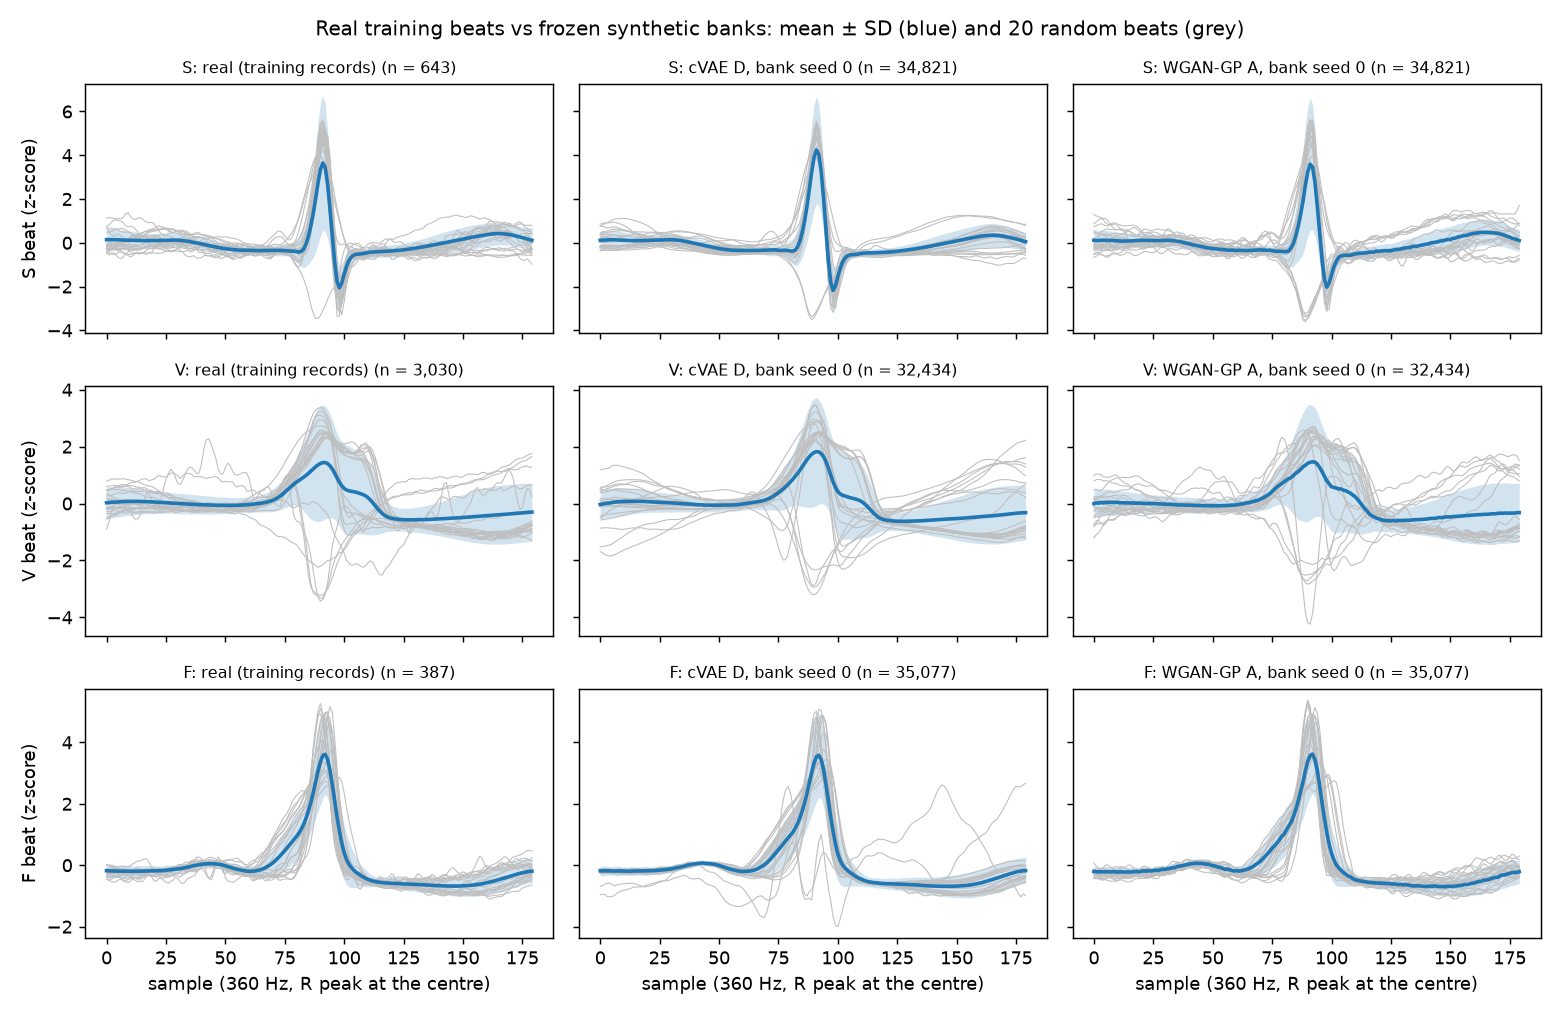
\includegraphics[width=\linewidth]{phase3_gate/banks.png}\caption{Real training beats beside the frozen
synthetic banks of the chosen cVAE and WGAN-GP variants (bank seed 0) for S, V and F: mean $\pm$ SD (blue) and 20 random beats (grey).
Both generators reproduce the class-average shape; the real beats vary more from patient to patient than the synthetic ones
suggest.}\label{fig:banks}\end{figure}

\subsection{Augmentation policy and the comparison grid (phase 4)}
Four policies decide how many synthetic beats each rare class receives: balancing to the training N count, a fraction of the N count, a
multiple of the class's real count, and a fraction of the N count drawn from a DTW-screened pool. The policy was chosen on validation with
both banks, subject to a limit of 0.01 on the loss of N recall (Table~\ref{tab:policy}). The full grid then trains six conditions (none,
class-weighted loss with weights $(n_{\max}/n_c)^{\gamma}$, random oversampling, SMOTE, cVAE and WGAN-GP) at three strengths each (one
for none), for both classifiers and three seeds; classifier seed $s$ uses bank seed $s$, and validation and test stay entirely real. The
strength of each condition and the best generative condition per classifier were fixed on validation (Figure~\ref{fig:strength}) before
the test records were read.
\begin{table}[htbp]\centering\small\adjustbox{max width=\linewidth}{% Generated by python -m ecgaug.paper from: results/phase4_augmentation_policy/A.json, results/phase4_augmentation_policy/B.json, results/phase4_augmentation_policy/C.json, results/phase4_augmentation_policy/D.json
\begin{tabular}{llrrrl}
\toprule
Variant & Policy & Pilot strength & S F1 (val., 2 banks) & $\Delta$ N recall & Within limit \\
\midrule
A & balance\_to\_n & None & 0.396 & +0.042 & no \\
B & fraction\_of\_n & 0.5 & 0.446 & +0.016 & no \\
C & multiple\_of\_real & 2.0 & 0.401 & +0.035 & no \\
D & fraction\_of\_n\_screened & 0.5 & 0.383 & -0.006 & yes \\
\bottomrule
\end{tabular}
}\caption{Augmentation
policies (pilot, validation).}\label{tab:policy}\end{table}
\begin{figure}[htbp]\centering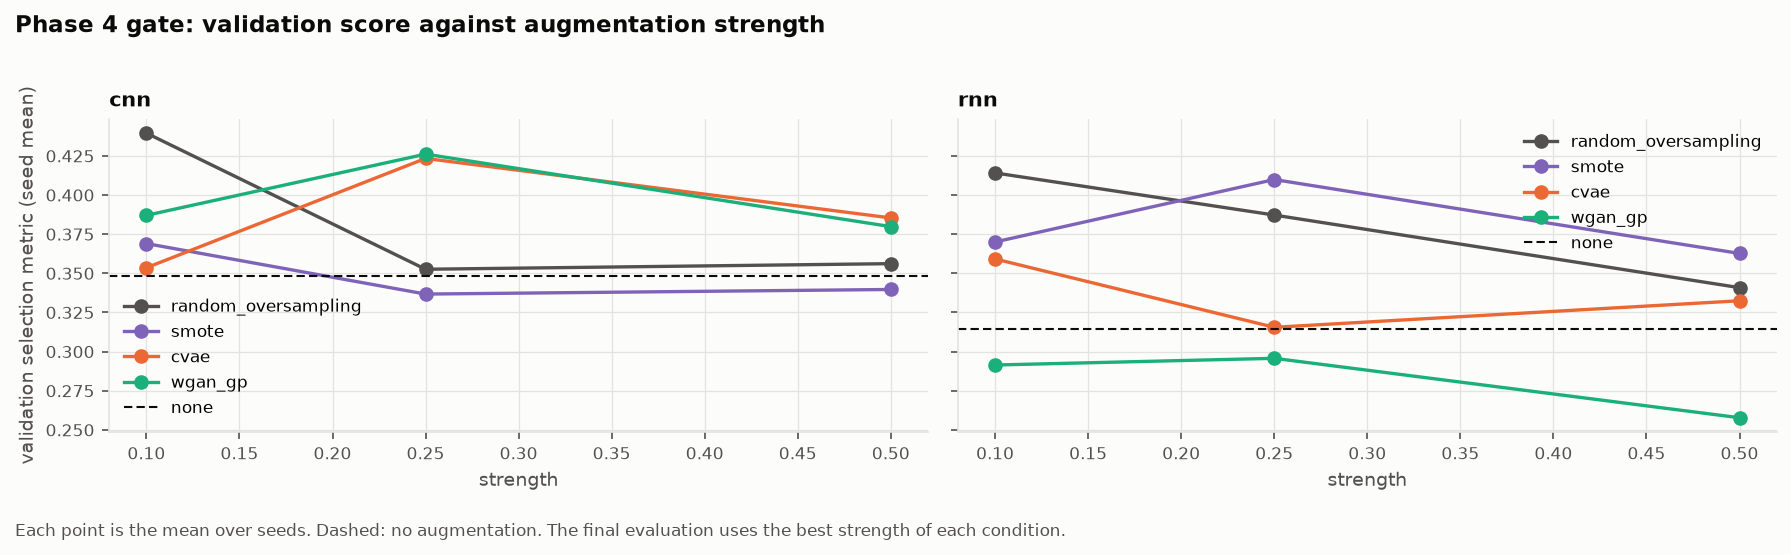
\includegraphics[width=\linewidth]{phase4_gate/strength_curves.png}\caption{The validation selection
score (mean over seeds) against augmentation strength for each condition and classifier; dashed, no augmentation. Each condition enters
the final evaluation at its best strength.}\label{fig:strength}\end{figure}

\subsection{Saliency maps and notes (phase 5)}
Four saliency methods were compared for each classifier: Grad-CAM~\cite{selvaraju2016gradcam}, integrated
gradients~\cite{sundararajan2017ig}, SmoothGrad~\cite{smilkov2017smoothgrad} and occlusion. A method is faithful when deleting the
samples it marks as important lowers the predicted probability faster than deleting random samples, and stable when maps from different
seeds agree; the rule weighed both (Table~\ref{tab:explain}). Each map is summarised as its share inside fixed P, QRS, ST and T windows
around the R peak, the clinician's vocabulary for the parts of a beat. For the notes, four generators were compared: a deterministic
template, and three LLM variants (a constrained prompt, few-shot examples with a fixed output schema, and a fact-check-and-regenerate loop
that falls back to the template). The fact checker verifies that every class name, number and segment in a note appears in the input, that
the disclaimer is present, and that a low-confidence note (top probability below 0.6) asks for clinician review; the hard gate is zero
unsupported claims over 50 validation cases.

\section{Pre-registered results}\label{sec:results}
Table~\ref{tab:hypotheses} gives the verdict on each pre-registered hypothesis; the subsections below give the evidence.
\begin{table}[htbp]\centering\small\adjustbox{max width=\linewidth}{% Generated by python -m ecgaug.paper from the result files
\begin{tabular}{lp{5.2cm}lp{5.2cm}}
\toprule
Hypothesis & Statement & Verdict & Evidence \\
\midrule
H1 & confirmatory: a generative condition improves test rare-class macro-F1 over none (Holm, 4 tests) & not supported & no confirmatory comparison significant \\
H1b & exploratory: gains larger for F than for S & mixed & F gain larger than S gain in 2 of 4 generative conditions \\
H1c & secondary: generative beats SMOTE, random oversampling and class-weighted loss & not supported & 0 of 6 comparisons of the best generative condition with a baseline significant \\
H2 & exploratory: intra-patient evaluation inflates the baseline and the gains & not consistent & inflation of the baseline +0.748; larger intra-patient gain for 0 of 2 generators \\
H3 & exploratory: a quality metric predicts the downstream gain & not supported & 0 of 5 metrics with an interval excluding zero \\
H4 & exploratory: augmented models are at least as faithful as the baseline & mixed & augmented faithfulness at least the baseline's in 1 of 4 model pairs \\
\bottomrule
\end{tabular}
}\caption{Pre-registered
hypotheses and their verdicts.}\label{tab:hypotheses}\end{table}

\subsection{Does generative augmentation help?}
For the cnn (shallow cnn), training without augmentation reached a test rare-class macro-F1 of 0.088 (95\% CI 0.037 to 0.194). cVAE augmentation (strength 0.25) did not detectably change it: difference +0.025 (95\% CI $-$0.018 to +0.047), Holm-adjusted $p=1.000$. WGAN-GP augmentation (strength 0.1) did not detectably change it: difference $-$0.009 (95\% CI $-$0.045 to +0.015), Holm-adjusted $p=1.000$.

In the secondary family for the cnn (best generative condition on validation: cVAE), cVAE was not detectably different from WGAN-GP (+0.034 (95\% CI $-$0.002 to +0.068), Holm-adjusted $p=0.550$); cVAE was not detectably different from SMOTE (+0.044 (95\% CI $-$0.029 to +0.072), Holm-adjusted $p=1.000$); cVAE was not detectably different from class-weighted loss (+0.001 (95\% CI $-$0.041 to +0.042), Holm-adjusted $p=1.000$); cVAE was not detectably different from random oversampling ($-$0.022 (95\% CI $-$0.074 to +0.010), Holm-adjusted $p=1.000$).

For the rnn (bilstm), training without augmentation reached a test rare-class macro-F1 of 0.075 (95\% CI 0.014 to 0.232). cVAE augmentation (strength 0.1) did not detectably change it: difference $-$0.002 (95\% CI $-$0.100 to +0.032), Holm-adjusted $p=1.000$. WGAN-GP augmentation (strength 0.5) did not detectably change it: difference $-$0.006 (95\% CI $-$0.138 to +0.035), Holm-adjusted $p=1.000$.

In the secondary family for the rnn (best generative condition on validation: cVAE), cVAE was not detectably different from WGAN-GP (+0.004 (95\% CI $-$0.027 to +0.065), Holm-adjusted $p=1.000$); cVAE was not detectably different from SMOTE ($-$0.013 (95\% CI $-$0.067 to +0.016), Holm-adjusted $p=1.000$); cVAE was not detectably different from class-weighted loss (+0.012 (95\% CI $-$0.047 to +0.039), Holm-adjusted $p=1.000$); cVAE was not detectably different from random oversampling ($-$0.016 (95\% CI $-$0.059 to +0.016), Holm-adjusted $p=1.000$).

H1 (confirmatory) is not supported: no generative condition improved the primary metric after Holm correction.

Without record 202 (the DS2 record of the subject of DS1 record 201) the confirmatory conclusions are unchanged.

Per class (exploratory, H1b; differences of test F1 point estimates against no augmentation): cVAE with the cnn: F +0.025, S +0.025; WGAN-GP with the cnn: F $-$0.027, S +0.008; cVAE with the rnn: F +0.007, S $-$0.011; WGAN-GP with the rnn: F +0.013, S $-$0.025.
 Figure~\ref{fig:forest} shows each pre-registered comparison.
\begin{table}[htbp]\centering\small\adjustbox{max width=\linewidth}{\begin{tabular}{llrrr}
\toprule
Architecture & Condition & Strength & Rare macro-F1 [95\% CI] & N recall \\
\midrule
cnn & none & -- & 0.088 [0.037, 0.194] & 0.962 \\
cnn & class weighted & 0.5 & 0.113 [0.057, 0.207] & 0.933 \\
cnn & random oversampling & 0.1 & 0.136 [0.061, 0.247] & 0.844 \\
cnn & smote & 0.1 & 0.070 [0.025, 0.172] & 0.985 \\
cnn & cvae & 0.25 & 0.113 [0.049, 0.217] & 0.938 \\
cnn & wgan gp & 0.1 & 0.079 [0.033, 0.164] & 0.955 \\
rnn & none & -- & 0.075 [0.014, 0.232] & 0.961 \\
rnn & class weighted & 0.75 & 0.061 [0.022, 0.168] & 0.865 \\
rnn & random oversampling & 0.1 & 0.090 [0.028, 0.196] & 0.883 \\
rnn & smote & 0.1 & 0.086 [0.025, 0.206] & 0.894 \\
rnn & cvae & 0.1 & 0.073 [0.035, 0.157] & 0.926 \\
rnn & wgan gp & 0.5 & 0.069 [0.027, 0.156] & 0.857 \\
\bottomrule
\end{tabular}
}\caption{Test results
per condition (95\% record-level CI).}\label{tab:test}\end{table}
\begin{figure}[htbp]\centering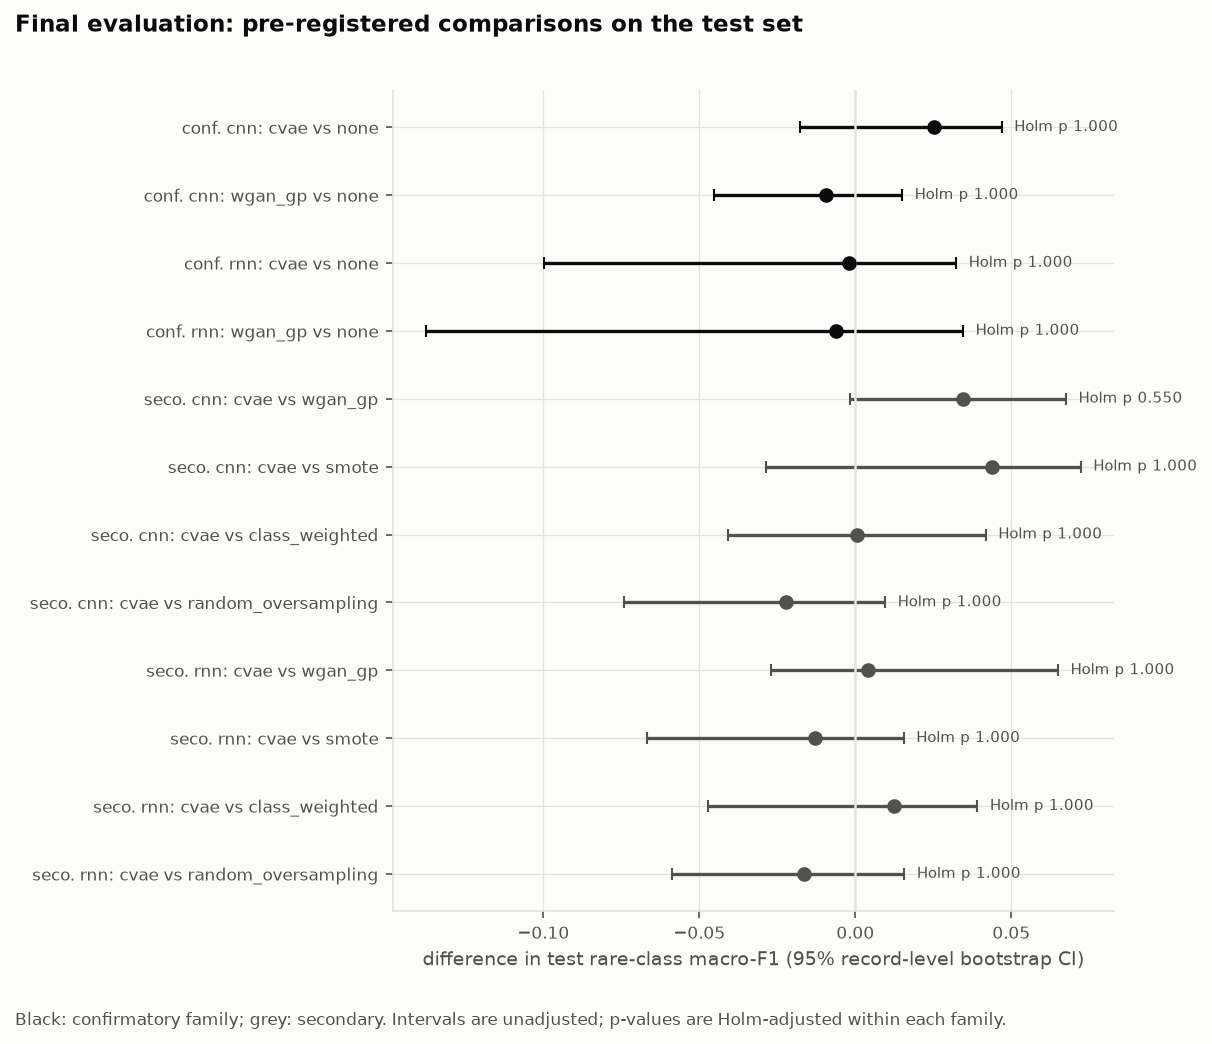
\includegraphics[width=0.9\linewidth]{final_eval/forest.png}\caption{The pre-registered comparisons on
the test records: difference in rare-class macro-F1 with 95\% record-level intervals (black, confirmatory; grey, secondary).}
\label{fig:forest}\end{figure}

\paragraph{Where the errors are.} The test rare beats sit in very few patients: record 232 holds 1,381 of the 1,836 test S beats, and record 213 holds 362 of the 388 test F beats. Across the 12 models of Table~\ref{tab:test} (seed means), S recall on record 232 ranged from 0.00 to 0.10, and F recall on record 213 ranged from 0.00 to 0.35, so these two records set most of the primary metric. The cnn without augmentation labelled 1,367 of 1,836 S beats and 333 of 388 F beats as normal (exploratory). With seed 0, S beats it found were more premature than S beats it called normal (median ratio of the previous RR interval to the local mean 0.57 against 0.72).
 In clinical terms the models miss most of the early
atrial beats of one patient and most of the fusion beats of another. Figure~\ref{fig:per-record} gives recall per test record.
\begin{figure}[htbp]\centering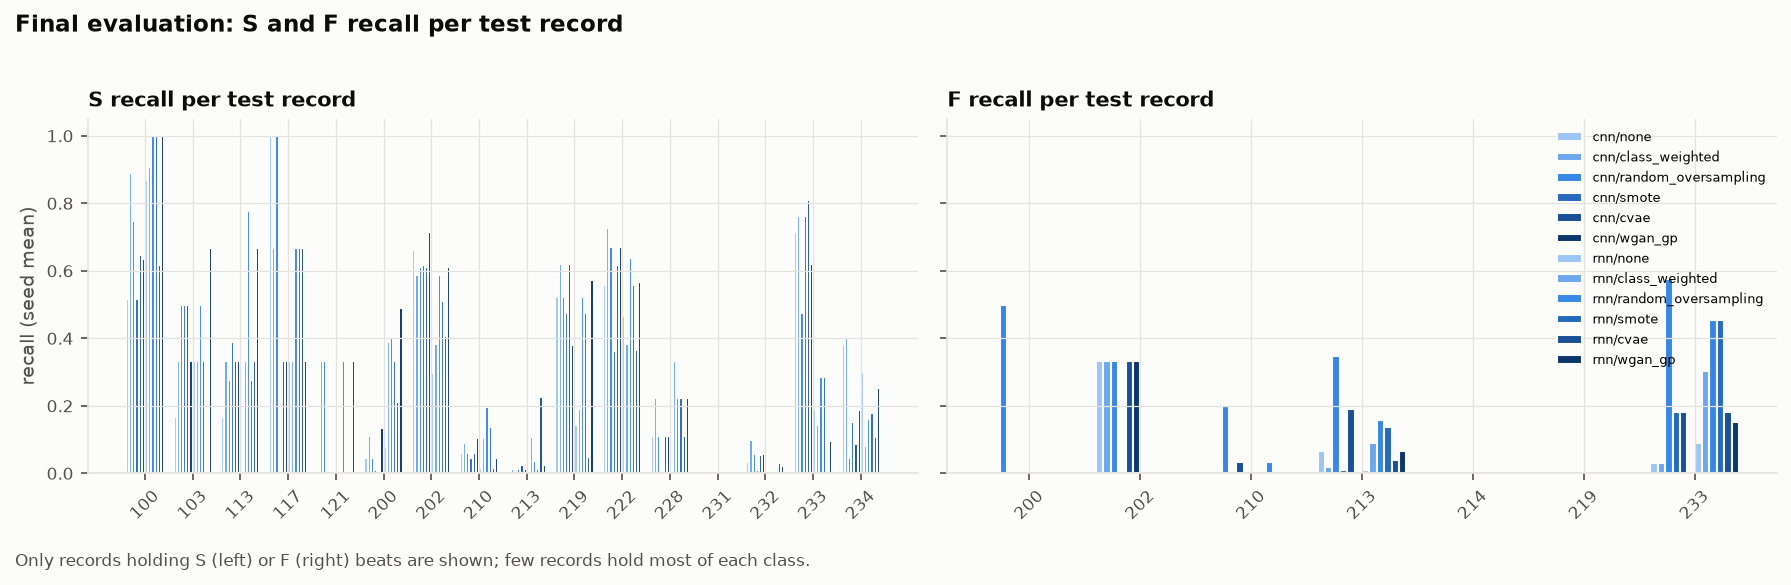
\includegraphics[width=\linewidth]{final_eval/per_record_S_F.png}\caption{S and F recall per test
record and model (seed means); grey cells are records without beats of the class.}\label{fig:per-record}\end{figure}

\subsection{How much does testing on seen patients inflate the score?}
With the same pipeline on a random beat-level split that pools DS1 and DS2 (44 of 44 records have beats in both training and test), the cnn without augmentation reached a rare-class macro-F1 of 0.837 $\pm$ 0.026 (mean $\pm$ SD over seeds), against 0.088 (95\% CI 0.037 to 0.194) under the inter-patient protocol: evaluated intra-patient, the primary metric was raised by 0.748. The apparent gain of cVAE over none was $-$0.017 intra-patient and +0.025 (95\% CI $-$0.018 to +0.047) inter-patient. The apparent gain of WGAN-GP over none was $-$0.052 intra-patient and $-$0.009 (95\% CI $-$0.045 to +0.015) inter-patient.

\begin{table}[htbp]\centering\small\adjustbox{max width=\linewidth}{% Generated by python -m ecgaug.paper from: results/phase4_leakage_audit/summary.json, results/final_eval/summary.json
\begin{tabular}{lrrrr}
\toprule
Condition & Intra-patient (mean $\pm$ SD) & Inter-patient [95\% CI] & Gain, intra & Gain, inter [95\% CI] \\
\midrule
none & 0.837 $\pm$ 0.026 & 0.088 [0.037, 0.194] & -- & -- \\
cvae & 0.820 $\pm$ 0.034 & 0.113 [0.049, 0.217] & -0.017 & 0.025 [-0.018, 0.047] \\
wgan\_gp & 0.785 $\pm$ 0.060 & 0.079 [0.033, 0.164] & -0.052 & -0.009 [-0.045, 0.015] \\
\bottomrule
\end{tabular}
}\caption{Rare-class
macro-F1 of the cnn with a random beat-level split of DS1 and DS2 (intra-patient) and on DS2 (inter-patient). Run after the final
evaluation; never used for any decision.}\label{tab:audit}\end{table}
\begin{figure}[htbp]\centering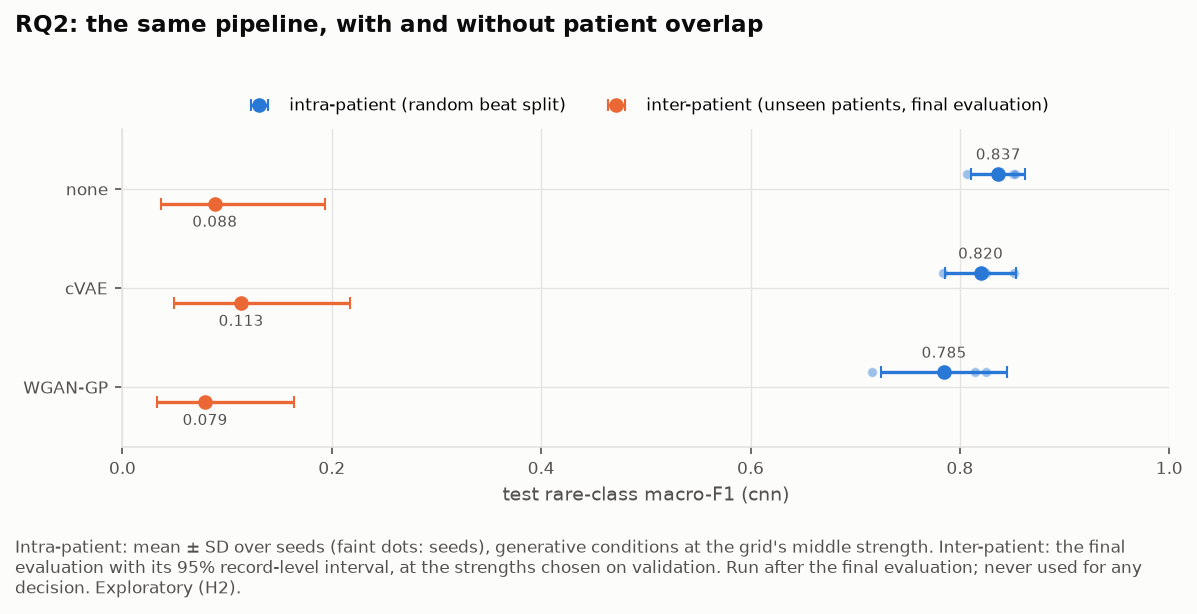
\includegraphics[width=\linewidth]{phase4_leakage_audit/intra_vs_inter.png}\caption{The cnn with and
without patient overlap between training and test.}\label{fig:leakage}\end{figure}

\subsection{Do quality metrics predict the benefit?}
Across 96 checkpoints of 24 generator runs (exploratory; intervals resample runs), no fidelity or diversity metric had an interval excluding zero. The others: dtw ($\rho=-0.20$, 95\% CI $-$0.44 to +0.06), spectral ($\rho=-0.00$, 95\% CI $-$0.25 to +0.23), diversity ratio ($\rho=-0.12$, 95\% CI $-$0.34 to +0.13), memorization fraction ($\rho=+0.18$, 95\% CI $-$0.07 to +0.40), c2st accuracy ($\rho=+0.04$, 95\% CI $-$0.20 to +0.25).
 Figure~\ref{fig:quality-gain} shows each metric against the gain.
\begin{figure}[htbp]\centering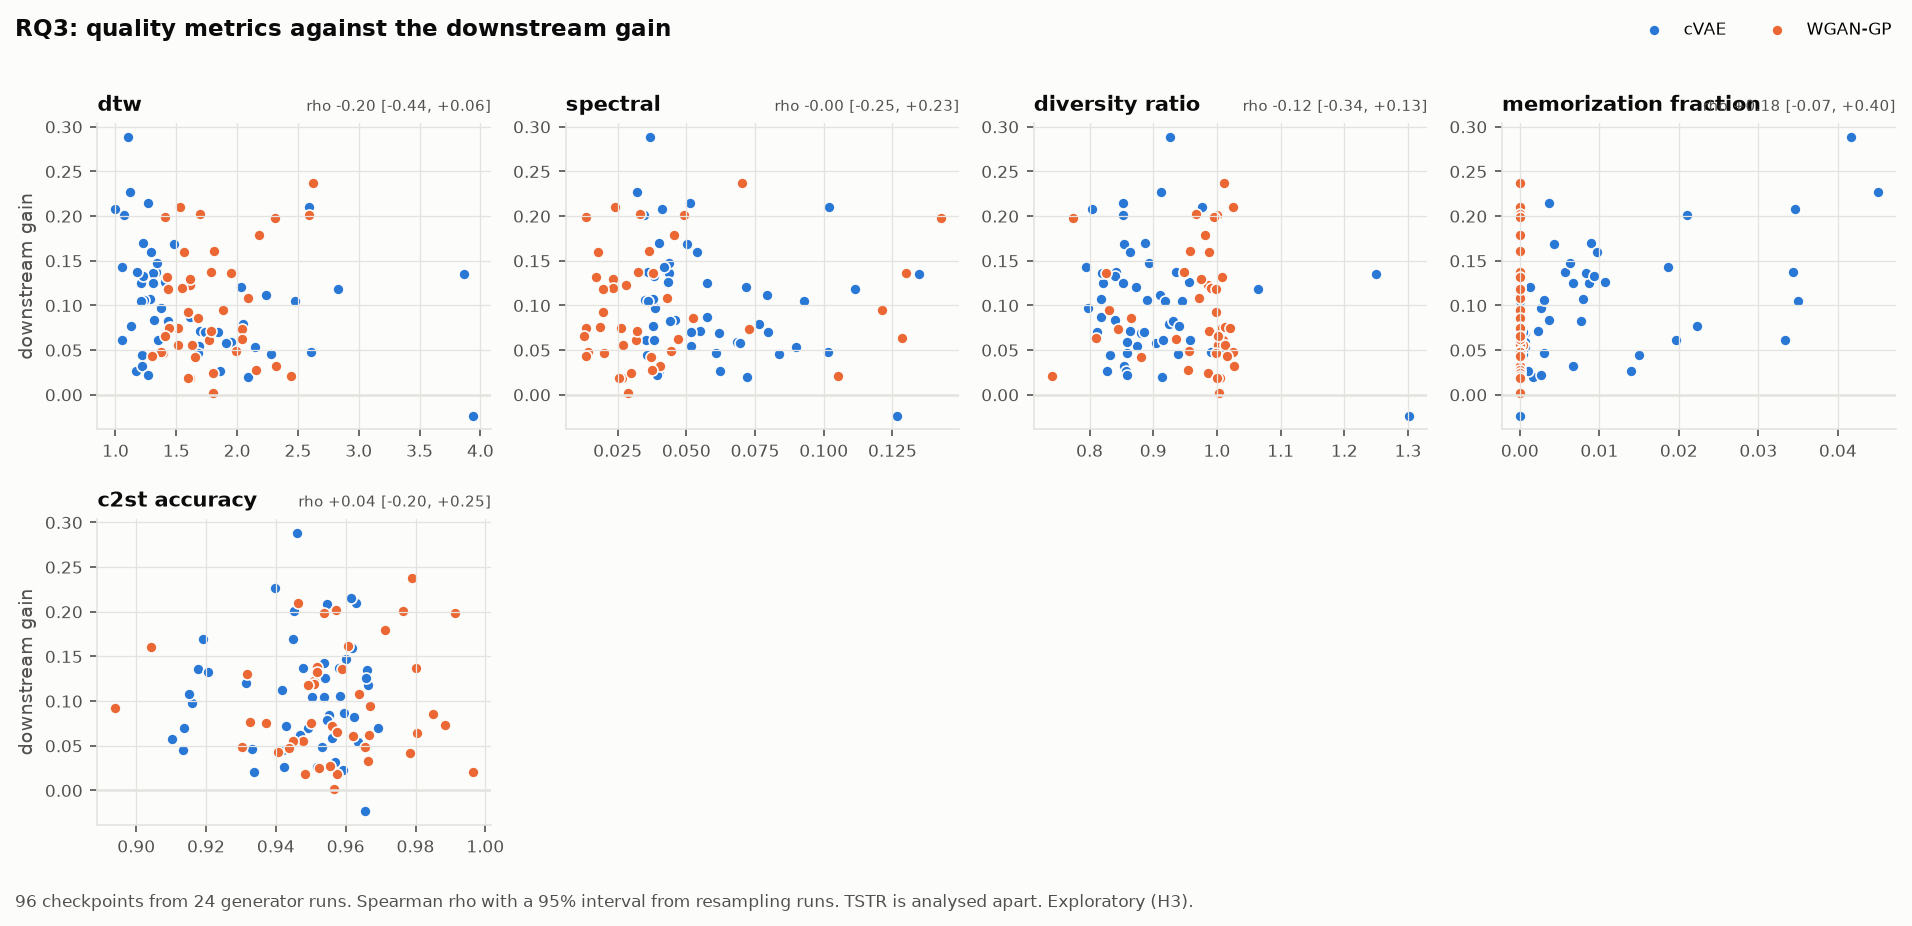
\includegraphics[width=\linewidth]{phase4_quality_vs_gain/quality_vs_gain.png}\caption{Each quality
metric against the downstream gain of the same generator checkpoint, with Spearman's $\rho$ and its 95\% interval.}
\label{fig:quality-gain}\end{figure}

\subsection{Does augmentation change what the classifier looks at?}
For the cnn, the rule chose Grad-CAM. Its faithfulness gain over random deletion was +0.1522 for none, +0.1175 for cVAE, +0.1572 for WGAN-GP. The cVAE model put 0.48 of its saliency mass in the QRS window on synthetic S, V and F beats against 0.34 on real ones (a shift that may indicate reliance on synthetic artifacts). The WGAN-GP model put 0.40 of its saliency mass in the QRS window on synthetic S, V and F beats against 0.37 on real ones.

For the rnn, the rule chose occlusion. Its faithfulness gain over random deletion was +0.1129 for none, +0.0541 for cVAE, +0.0917 for WGAN-GP. The cVAE model put 0.10 of its saliency mass in the QRS window on synthetic S, V and F beats against 0.14 on real ones. The WGAN-GP model put 0.12 of its saliency mass in the QRS window on synthetic S, V and F beats against 0.15 on real ones.

\begin{table}[htbp]\centering\small\adjustbox{max width=\linewidth}{% Generated by python -m ecgaug.paper from: results/phase5_explainability/A.json, results/phase5_explainability/B.json, results/phase5_explainability/C.json, results/phase5_explainability/D.json
\begin{tabular}{llrrrr}
\toprule
Variant & Method & cnn faithfulness gain & cnn stability & rnn faithfulness gain & rnn stability \\
\midrule
A & gradcam & 0.1423 & 0.389 & n/a & n/a \\
B & integrated\_gradients & 0.0279 & 0.558 & 0.0600 & 0.610 \\
C & smoothgrad & 0.0382 & 0.401 & 0.0297 & 0.498 \\
D & occlusion & 0.0988 & 0.747 & 0.0862 & 0.515 \\
\bottomrule
\end{tabular}
}\caption{Saliency
methods: faithfulness gain over random deletion and stability across seeds.}\label{tab:explain}\end{table}
\begin{figure}[htbp]\centering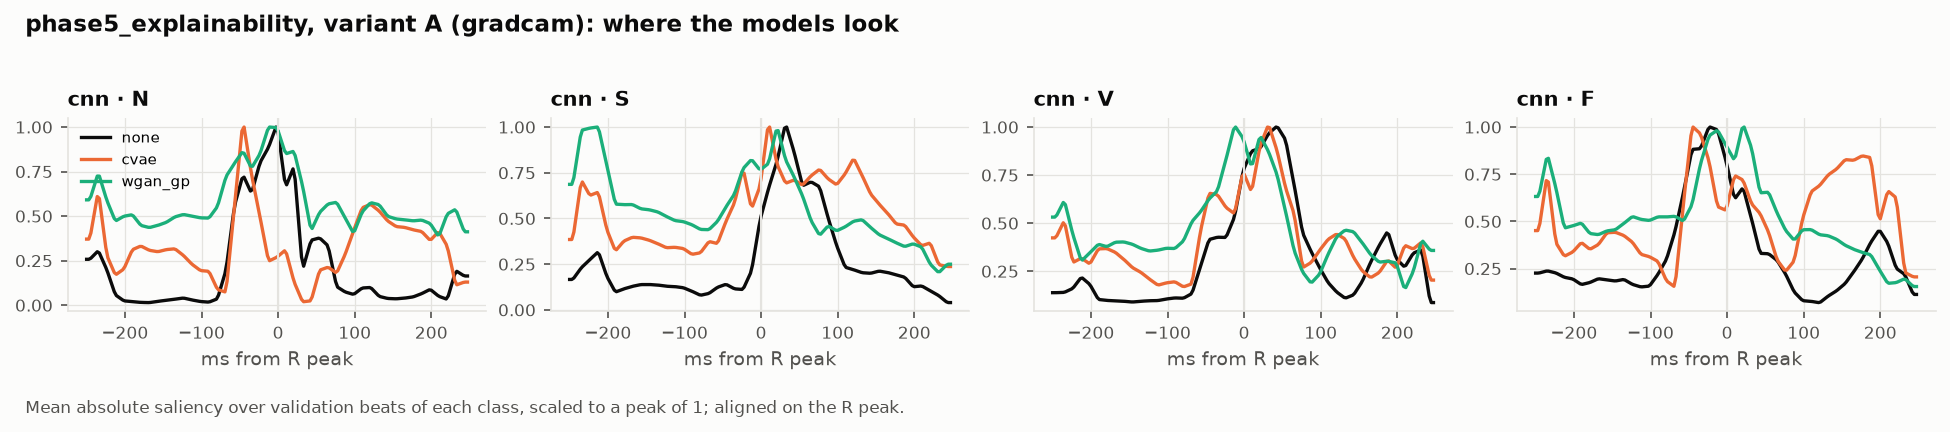
\includegraphics[width=\linewidth]{phase5_explainability/A/class_average_saliency.png}\caption{Where
the cnn looks (Grad-CAM, validation beats): the mean saliency of each class without augmentation and with each generator.}
\label{fig:saliency}\end{figure}

\subsection{Notes}
The rule chose note generator C (As B plus two few-shot examples and a fixed JSON output schema, rendered to a note). Over 50 validation cases, 16 of them low-confidence, it produced 0 unsupported claims, with coverage 1.00 of the required parts. Variants run: A, B, C, D.
 The LLM variants use Gemini 3.5 Flash-Lite on Google's free tier (decisions A21 and A23 in
\texttt{docs/DECISIONS.md}); the generator receives only the JSON object, built from the public database.
\begin{table}[htbp]\centering\small% Generated by python -m ecgaug.paper from: results/phase5_clinical_notes/A.json, results/phase5_clinical_notes/B.json, results/phase5_clinical_notes/C.json, results/phase5_clinical_notes/D.json
\begin{tabular}{lrrrr}
\toprule
Variant & Unsupported claims & Coverage & Fell back & Latency (s) \\
\midrule
A & 0 & 1.00 & 0 & 0.00 \\
B & 0 & 0.98 & 0 & 3.05 \\
C & 0 & 1.00 & 0 & 2.63 \\
D & 0 & 0.98 & 0 & 2.17 \\
\bottomrule
\end{tabular}
\caption{Note generators: unsupported claims and
coverage.}\label{tab:notes}\end{table}

\section{Follow-up analyses}\label{sec:posthoc}
\begin{figure}[htbp]\centering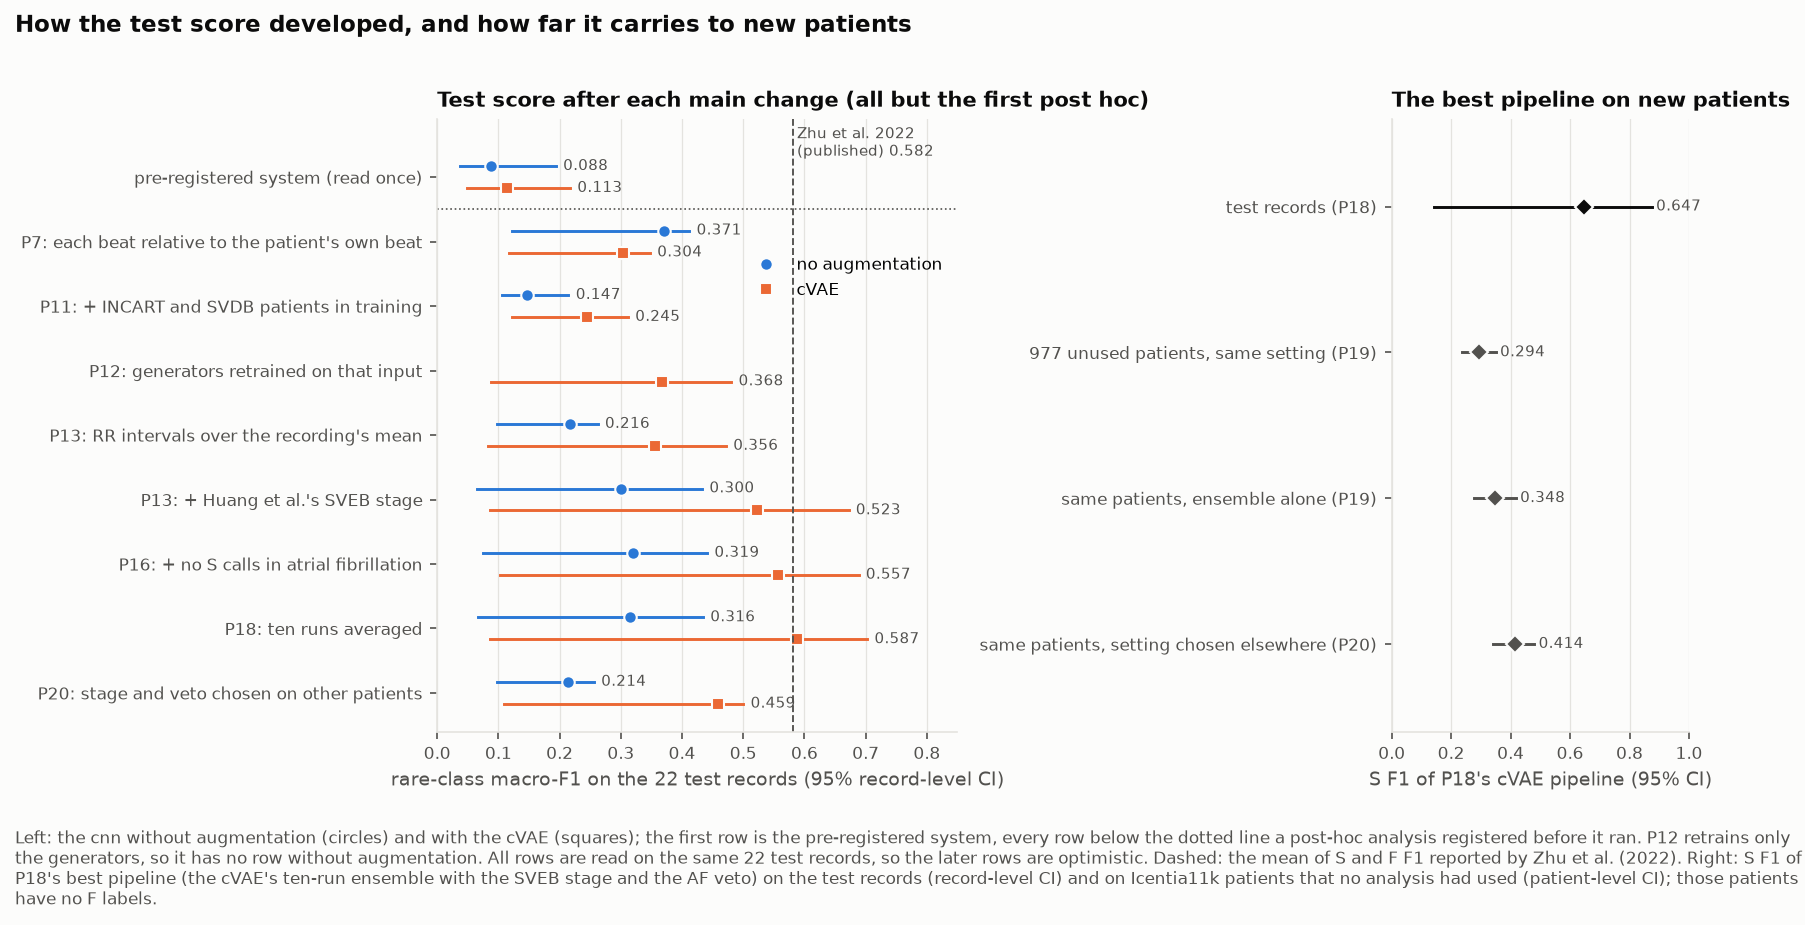
\includegraphics[width=\linewidth]{report/progress.png}\caption{How the test score developed through
the main follow-up analyses, and how far the best pipeline carries to new patients.}\label{fig:progress}\end{figure}
\begin{table}[htbp]\centering\small
\caption{The post-hoc analyses (pre-registration versions 4 to 21), each reported apart from the primary results. Numbers are test rare-class macro-F1 unless stated.}\label{tab:posthoc}
\begin{tabular}{@{}lp{0.3\linewidth}p{0.55\linewidth}@{}}
\toprule
 & question & finding \\
\midrule
P1 & Is the cnn simply weak? & RR-only LDA 0.022 vs cnn 0.088 \\
P2 & Does it hold on other databases? & INCART: generative vs none lowered in 1, did not detectably change in 3 of 4; SVDB: generative vs none did not detectably change in 3, improved in 1 of 4 \\
P3 & Are three seeds enough? & five seeds: 0 verdicts changed \\
P4 & Does the audit depend on its split? & intra-patient 0.777--0.837 vs 0.088 inter-patient \\
P5 & A better RR feature? & test v2 $-$ v1 $-$0.042 to +0.046; generative vs none did not detectably change in 4 of 4 \\
P6 & Patient-relative beats? & validation S F1 v3 $-$ v2: cnn +0.122, rnn $-$0.125; not adopted \\
P7 & A stronger cnn? & test cnn none 0.371 (v1 0.088); generative vs none did not detectably change in 2 of 2 \\
P8 & Do synthetic beats add patients? & synthetic S beats nearest to record 209: 0.61 (real 0.60) \\
P9 & Augmentation that adds patients? & generative transfer vs none did not detectably change in 4 of 4 \\
P10 & Per-patient normalization in the network? & v1/cnn +0.162; v1/rnn $-$0.067; p7/cnn $-$0.031 validation S F1; test: adaptation did not detectably change in 1 of 1, generative vs none did not detectably change in 2 of 2 \\
P11 & More training patients? & cnn none 0.147 vs DS1 only: did not detectably change in 1 of 1; each condition vs none: did not detectably change in 4 of 4; best class-weighted loss 0.407 \\
P12 & Generators trained on what the cnn sees? & cVAE 0.368, WGAN-GP 0.243; vs the same generator in P11: did not detectably change in 2 of 2; vs P11 none and oversampling: did not detectably change in 4 of 4 \\
\bottomrule
\end{tabular}
\end{table}
\begin{table}[htbp]\centering\small
\caption{The post-hoc analyses, continued.}
\begin{tabular}{@{}lp{0.3\linewidth}p{0.55\linewidth}@{}}
\toprule
 & question & finding \\
\midrule
P13 & RR intervals over the recording's mean? & none 0.147 to 0.216; best class-weighted loss 0.380; vs before: did not detectably change in 5 of 5; generative vs the others: did not detectably change in 6 of 6 \\
P14 & Many more training patients (Icentia11k)? & none 0.216 to 0.121; best cVAE 0.304; vs P13: did not detectably change in 4 of 4; cVAE vs the others: did not detectably change in 3 of 3 \\
P15 & A diffusion model as the generator? & diffusion 0.280; vs none and cVAE: did not detectably change in 2 of 2; vs class weights and oversampling: did not detectably change in 2 of 2 \\
P16 & An AF veto on the SVEB stage? & cVAE with the stage and veto 0.557; veto vs stage alone: improved in 2, did not detectably change in 4 of 6 \\
P17 & Diffusion trained five times longer? & 0.267; vs P15 and none: did not detectably change in 2 of 2 \\
P18 & Ten runs averaged per condition? & cVAE ensemble with the stage and veto 0.587 (best test score); ensemble vs single runs: did not detectably change in 5, improved in 1 of 6; cVAE vs the others: did not detectably change in 5 of 5 \\
P19 & The same pipeline on 977 new patients? & S F1 0.286--0.295 (no F label); ensemble vs single runs: did not detectably change in 1, improved in 5 of 6; cVAE vs the others: did not detectably change in 5 of 5 \\
P20 & Stage and veto chosen on other patients? & P19's patients S F1 0.378--0.419 with the chosen settings; chosen vs P19's setting: improved in 6 of 6; test cVAE 0.459, chosen vs P18's setting: did not detectably change in 6 of 6 \\
P21 & A physics loss in the generators (SimGANs)? & P19's patients: did not detectably change in 2 of 2; test: did not detectably change in 2 of 2; best the cVAE with the Euler loss 0.481 \\
P22 & A larger classifier (ResNet1D)? & P19's patients: did not detectably change in 1, improved in 2 of 3; test: did not detectably change in 3 of 3; best the ResNet with the cVAE 0.486 \\
P23 & A physics loss fitted to each beat? & P19's patients: improved in 1, did not detectably change in 1 of 2; test: did not detectably change in 2 of 2; best the cVAE with the fitted loss 0.465 \\
\bottomrule
\end{tabular}
\end{table}

After the final evaluation, 23 follow-up analyses (P1 to P23) asked why augmentation did not help and what would. Each was added to the pre-registration (versions 4 to 21) before it ran, and every read of the test records is logged: 18 reads after the final evaluation. Later scores on the test records are therefore optimistic and do not replace the pre-registered results, so two analyses scored the best pipeline on 977 Icentia11k patients~\cite{tan2022icentia} that no analysis had used. Table~\ref{tab:posthoc} lists every analysis with its numbers, and Figure~\ref{fig:progress} follows the test score through the main changes.

\paragraph{The pre-registered answer holds.} With five seeds instead of three, no pre-registered verdict changed (P3). On two other databases, St Petersburg INCART and the MIT-BIH Supraventricular Arrhythmia Database~\cite{goldberger2000}, generative augmentation was detectably better than no augmentation in 1 and worse in 1 of 8 comparisons (P2). With beats split at random, so that the same patients are in training and test, the same cnn reached 0.777 to 0.837 against 0.088 across patients (P4): much of what such splits measure is how well a model recognises patients it has seen.

\paragraph{The patient limits the model more than the class balance.} Giving the cnn each beat relative to the patient's own median beat (P6, Figure~\ref{fig:relative}), with nothing else changed, raised its test score without augmentation from 0.088 to 0.371 (P7), more than any rebalancing method did. The synthetic S beats came from the same few patients as the real ones: 0.61 of them were nearest to a beat of record 209, against 0.60 of the real training S beats (P8, Figure~\ref{fig:synthetic-patients}), so the generators added beats but not patients. Methods that act on the patient were then tested: moving the deviation of each rare beat onto other patients' normal beats (P9), normalising each patient inside the network (P10), and adding the INCART and SVDB patients (P11) or 400 Icentia11k patients (P14) to training. Of their 10 test comparisons, none changed detectably; at this scale, adding patients did not by itself raise the score.

\paragraph{Timing identifies S beats, as it does for a cardiologist.} An S beat is recognised mainly by coming early for the patient's own rhythm (Section~\ref{sec:medical}). In P13, dividing the RR intervals by the recording's mean RR interval, as published methods do, did not detectably change the cnn's test score in any of the 5 conditions (without augmentation 0.147 to 0.216, S F1 0.294 to 0.399); with Huang et al.'s rule on top, which uses the same feature directly, S F1 reached 0.531 to 0.578 (sensitivity 0.920 to 0.955) and the cVAE's rare-class macro-F1 0.523 (descriptive, not tested). Figure~\ref{fig:rr-reference} shows what each reference makes of the training-side recordings. In P16, undoing the rule's S calls inside atrial fibrillation, found by a detector that reads only beat times, raised rare-class macro-F1 in all 6 conditions (by 0.018 to 0.034; every 95\% interval above zero; detectable after Holm correction in 2), by removing false S calls: the cVAE went from 0.523 to 0.557 (S F1 0.572 to 0.640, F F1 0.474).

\paragraph{Better generators and a larger classifier did not change the answer.} A class-conditional diffusion model (P15), the same model trained five times longer (P17), the physics loss of SimGANs, which scores generated beats with an ECG simulator (P21), and a physics loss fitted to each generated beat (P23) were each compared on the test records with the generator they replace or with no augmentation; of these 8 comparisons, none changed detectably. A ResNet with 6.7 times the cnn's parameters (P22) raised supraventricular F1 on the unused patients in 2 of 3 comparisons; of its 3 comparisons on the test records, none changed detectably.

\paragraph{The best pipeline, and how far to trust it.} In P18, averaging the class probabilities of ten independently trained runs per condition changed rare-class macro-F1 by $-$0.004 to +0.099 against P16's single runs (after Holm correction: raised it in 1 of 6 conditions); the cVAE's ensemble reached 0.587, the highest test score of the study (S F1 0.647, F F1 0.527), against 0.557 for its single runs (not a detectable change, Holm-adjusted $p=1.000$). The mean of its S and F F1 is close to the best published inter-patient result we could check, 0.582 for Zhu et al.~\cite{zhu2022} (Section~\ref{sec:all-results}). The pipeline was designed after the test records had been read many times, so this score is optimistic. In P19, on 977 Icentia11k patients that no analysis had used, the same pipeline, unchanged, reached S F1 0.294 (95\% CI 0.237 to 0.350) and V F1 0.648 for the cVAE's ensemble with the stage and the veto, and S F1 0.348 for the ensemble alone. Icentia11k has no fusion label, so only S and V can be scored there. In P20, choosing the stage and the veto on 400 other Icentia11k patients picked \emph{stage 0.70, veto 0.80} for the cVAE, which took its S F1 on P19's patients from 0.294 to 0.414 (improved, Holm-adjusted $p=0.001$); on the test records its rare-class macro-F1 went from 0.587 with P18's setting to 0.459. On new patients, then, the pipeline's supraventricular F1 (0.294 and 0.414) stays well below the 0.647 measured on the test records.

\begin{figure}[htbp]\centering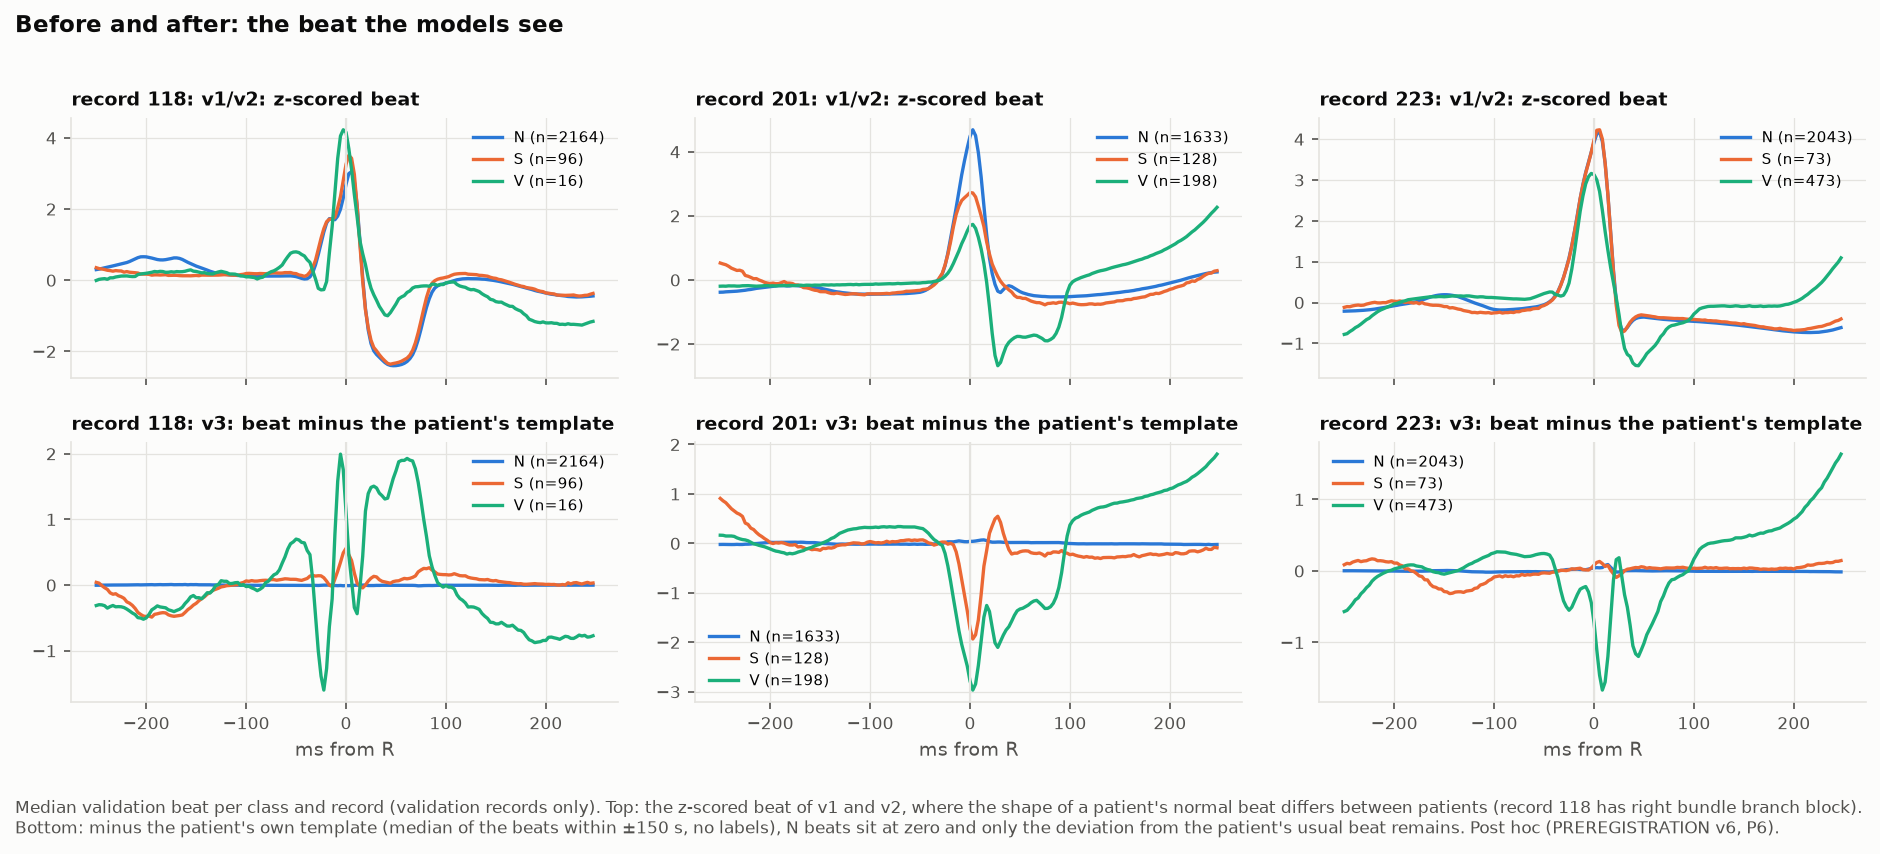
\includegraphics[width=\linewidth]{phase6_patient_template/input_v2_vs_v3.png}\caption{P6, validation
records only: the median beat per class as the models see it, z-scored (top) and minus the patient's own template (bottom). Record 118
has right bundle branch block, so its normal beats look unlike other patients'; minus the template, normal beats sit at zero and only the
deviation from the patient's usual beat remains.}\label{fig:relative}\end{figure}
\begin{figure}[htbp]\centering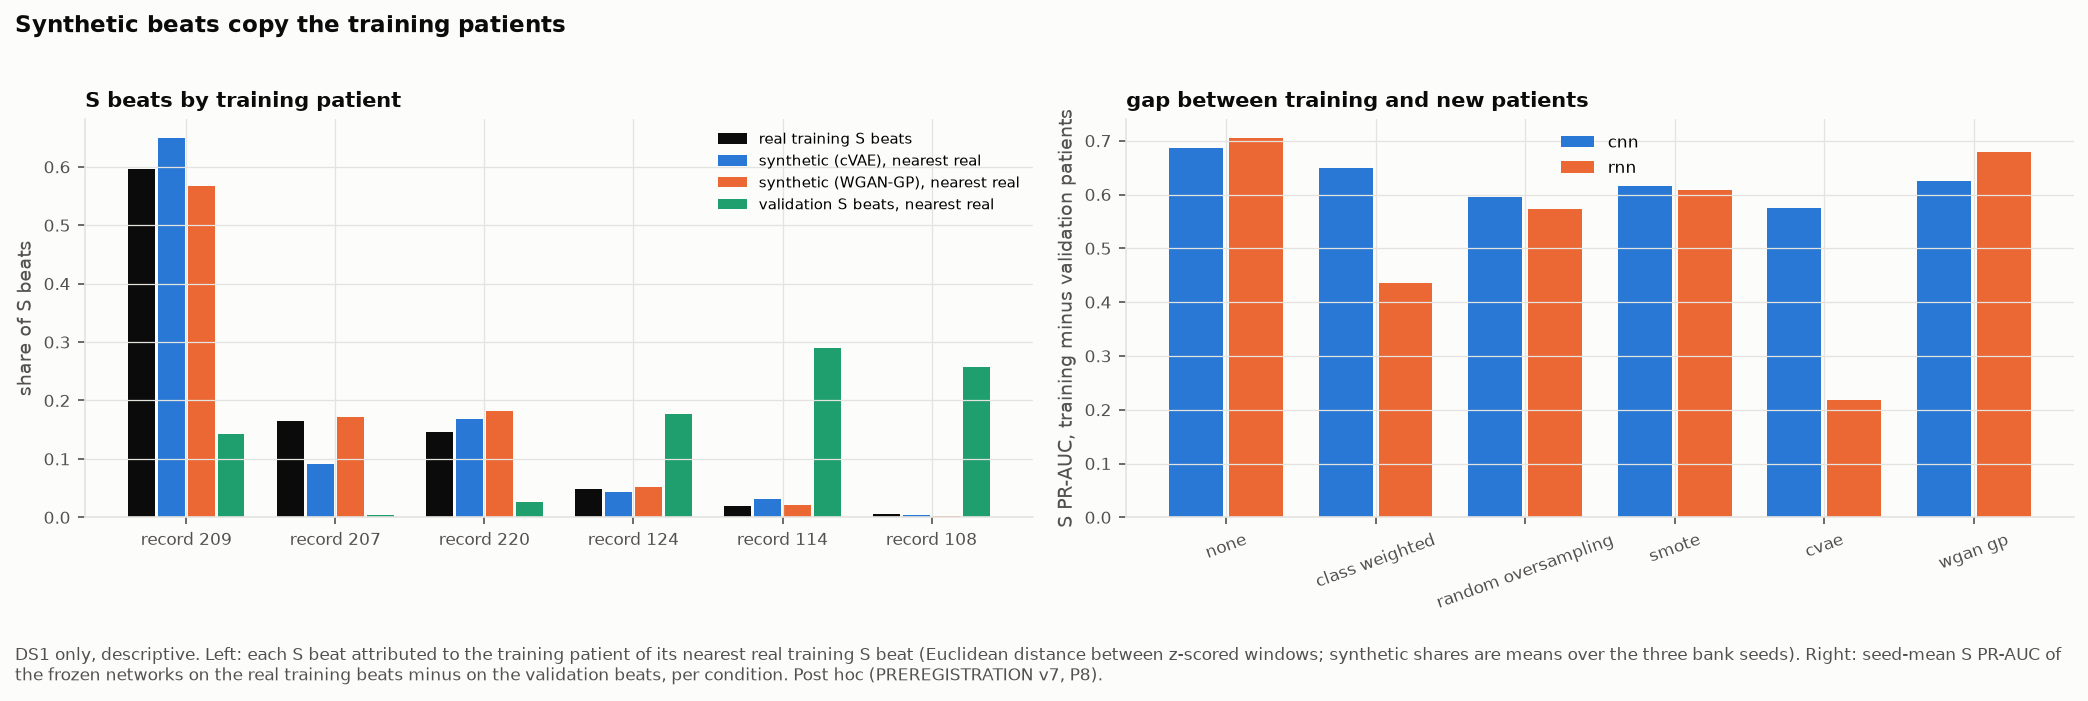
\includegraphics[width=\linewidth]{phase6_augmentation_mechanism/mechanism.png}\caption{P8, training and
validation records only: the share of S beats from each training patient, for the real beats and for the synthetic beats by their nearest
real beat (left), and the gap in S PR-AUC between the training and the validation patients for each condition (right).}
\label{fig:synthetic-patients}\end{figure}
\begin{figure}[htbp]\centering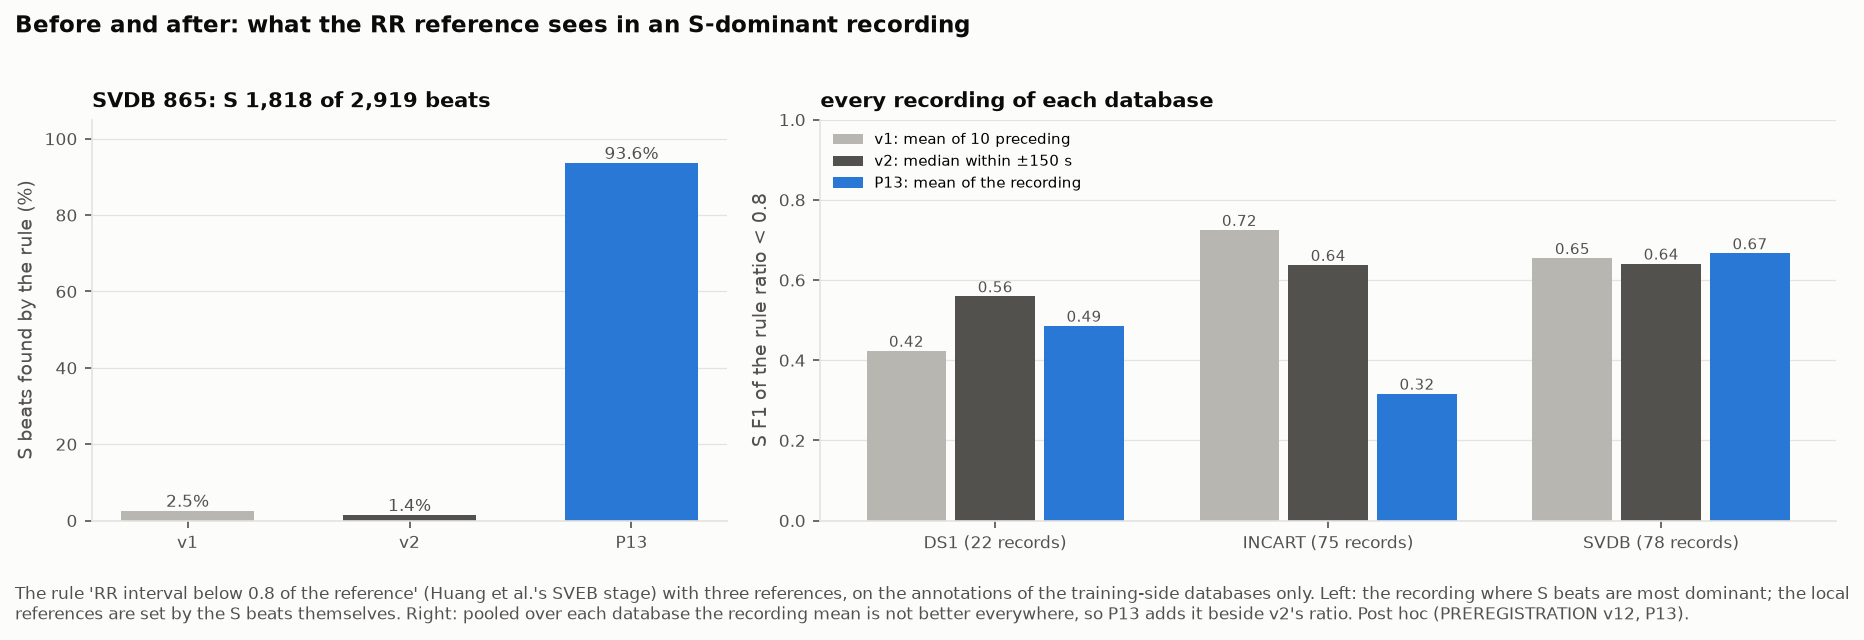
\includegraphics[width=\linewidth]{phase6_record_rr/check.png}\caption{P13, training-side annotations
only: the S beats that the rule ``RR interval below 0.8 of the reference'' finds with each reference, in the most S-dominant training
recording (left) and pooled over each database (right, S F1).}\label{fig:rr-reference}\end{figure}

\section{All results and the literature}\label{sec:all-results}
This section gathers every test metric that was computed, in the units of the AAMI standard: sensitivity (Se, recall), positive predictivity (+P, precision) and F1 per class, rare-class macro-F1 (the mean of S and F F1, the primary metric), macro-F1 over N, S, V and F, and accuracy. Table~\ref{tab:all-final} holds the twelve pre-registered models of the final evaluation, Table~\ref{tab:all-posthoc} the post-hoc ten-run pipelines and Table~\ref{tab:literature} published inter-patient results beside ours. The best value of each column is in bold.
\begin{table}[htbp]\centering\footnotesize\setlength{\tabcolsep}{3pt}
\adjustbox{max width=\linewidth}{\begin{tabular}{lrrrrrrrrrrrrrr}
\toprule
 & Rare F1 & Macro F1 & Acc. & N Se & N +P & S Se & S +P & S F1 & V Se & V +P & V F1 & F Se & F +P & F F1 \\
\midrule
cnn, none & 0.088 & 0.512 & 0.921 & 0.962 & 0.958 & 0.135 & 0.200 & 0.148 & \textbf{0.916} & 0.917 & \textbf{0.912} & 0.064 & \textbf{0.048} & 0.029 \\
cnn, class-weighted loss (0.5) & 0.113 & 0.512 & 0.895 & 0.933 & 0.954 & \textbf{0.213} & 0.249 & \textbf{0.223} & 0.858 & 0.927 & 0.878 & 0.019 & 0.004 & 0.003 \\
\textbf{cnn, random oversampling (0.1)} & \textbf{0.136} & 0.512 & 0.816 & 0.844 & 0.963 & 0.160 & 0.294 & 0.205 & 0.855 & 0.922 & 0.885 & \textbf{0.350} & 0.020 & \textbf{0.067} \\
cnn, SMOTE (0.1) & 0.070 & 0.502 & \textbf{0.935} & \textbf{0.985} & 0.949 & 0.088 & 0.218 & 0.121 & 0.855 & \textbf{0.966} & 0.901 & 0.014 & 0.039 & 0.018 \\
cnn, cVAE (0.25) & 0.113 & \textbf{0.517} & 0.899 & 0.938 & 0.957 & 0.152 & 0.201 & 0.173 & 0.873 & 0.931 & 0.893 & 0.185 & 0.039 & 0.054 \\
cnn, WGAN-GP (0.1) & 0.079 & 0.506 & 0.915 & 0.955 & 0.957 & 0.167 & 0.176 & 0.156 & 0.907 & 0.931 & 0.910 & 0.003 & 0.006 & 0.002 \\
rnn, none & 0.075 & 0.477 & 0.914 & 0.961 & 0.956 & 0.089 & \textbf{0.365} & 0.143 & 0.847 & 0.764 & 0.800 & 0.012 & 0.004 & 0.008 \\
rnn, class-weighted loss (0.75) & 0.061 & 0.436 & 0.831 & 0.865 & \textbf{0.964} & 0.090 & 0.143 & 0.104 & 0.879 & 0.607 & 0.712 & 0.092 & 0.010 & 0.018 \\
rnn, random oversampling (0.1) & 0.090 & 0.459 & 0.842 & 0.883 & 0.960 & 0.133 & 0.166 & 0.146 & 0.764 & 0.720 & 0.737 & 0.161 & 0.016 & 0.033 \\
rnn, SMOTE (0.1) & 0.086 & 0.466 & 0.852 & 0.894 & 0.955 & 0.116 & 0.200 & 0.147 & 0.788 & 0.757 & 0.770 & 0.141 & 0.014 & 0.026 \\
rnn, cVAE (0.1) & 0.073 & 0.386 & 0.852 & 0.926 & 0.924 & 0.100 & 0.206 & 0.132 & 0.375 & 0.648 & 0.473 & 0.041 & 0.007 & 0.015 \\
rnn, WGAN-GP (0.5) & 0.069 & 0.406 & 0.816 & 0.857 & 0.948 & 0.139 & 0.104 & 0.118 & 0.727 & 0.506 & 0.585 & 0.066 & 0.012 & 0.021 \\
\bottomrule
\end{tabular}}
\caption{The final evaluation on the 22 test records: every pre-registered model (mean of three seeds; strength in brackets). F Se, F +P, N +P and accuracy come from the seed-mean confusion matrix, the rest from the official summary.}\label{tab:all-final}
\end{table}
\begin{table}[htbp]\centering\footnotesize\setlength{\tabcolsep}{3pt}
\adjustbox{max width=\linewidth}{\begin{tabular}{lrrrrrrrr}
\toprule
 & Rare F1 & 95\% CI & S Se & S +P & S F1 & V F1 & F F1 & N Se \\
\midrule
P18: none, stage and veto (0.8, 0.95) & 0.316 & 0.066--0.434 & 0.918 & 0.481 & 0.631 & 0.934 & 0.000 & 0.959 \\
P18: class-weighted loss, stage and veto (0.8, 0.95) & 0.515 & 0.097--0.641 & 0.926 & 0.471 & 0.624 & 0.931 & 0.406 & 0.953 \\
P18: random oversampling, stage and veto (0.8, 0.95) & 0.541 & 0.103--0.700 & 0.931 & 0.479 & 0.632 & 0.918 & 0.451 & 0.955 \\
\textbf{P18: cVAE, stage and veto (0.8, 0.95)} & \textbf{0.587} & 0.086--0.702 & 0.914 & 0.500 & 0.647 & 0.936 & 0.527 & 0.962 \\
P18: WGAN-GP, stage and veto (0.8, 0.95) & 0.474 & 0.081--0.604 & \textbf{0.932} & 0.452 & 0.609 & 0.935 & 0.339 & 0.955 \\
P18: diffusion, stage and veto (0.8, 0.95) & 0.433 & 0.109--0.554 & 0.910 & 0.478 & 0.627 & 0.928 & 0.240 & 0.956 \\
P18: cVAE, the cnn alone & 0.387 & 0.073--0.492 & 0.211 & 0.296 & 0.247 & 0.936 & 0.527 & \textbf{0.979} \\
P20: none, setting chosen on Icentia11k & 0.214 & 0.098--0.256 & 0.441 & 0.416 & 0.428 & 0.934 & 0.000 & 0.974 \\
P20: class-weighted loss, setting chosen on Icentia11k & 0.369 & 0.125--0.434 & 0.336 & 0.327 & 0.332 & 0.931 & 0.406 & 0.968 \\
P20: random oversampling, setting chosen on Icentia11k & 0.449 & 0.134--0.553 & 0.477 & 0.420 & 0.447 & 0.918 & 0.451 & 0.970 \\
P20: cVAE, setting chosen on Icentia11k & 0.459 & 0.110--0.500 & 0.369 & 0.415 & 0.391 & 0.936 & 0.527 & 0.978 \\
P20: WGAN-GP, setting chosen on Icentia11k & 0.497 & 0.098--0.613 & 0.883 & \textbf{0.520} & \textbf{0.654} & 0.935 & 0.339 & 0.968 \\
P20: diffusion, setting chosen on Icentia11k & 0.331 & 0.137--0.381 & 0.434 & 0.411 & 0.422 & 0.928 & 0.240 & 0.972 \\
P21: cVAE with the Euler loss & 0.481 & 0.106--0.529 & 0.373 & 0.413 & 0.392 & 0.934 & \textbf{0.570} & 0.976 \\
P21: WGAN-GP with the Euler loss & 0.339 & 0.102--0.398 & 0.486 & 0.375 & 0.423 & 0.933 & 0.254 & 0.969 \\
P22: ResNet without augmentation & 0.270 & 0.141--0.347 & 0.301 & 0.405 & 0.345 & 0.926 & 0.194 & 0.976 \\
P22: ResNet with the cVAE & 0.486 & 0.149--0.529 & 0.436 & 0.508 & 0.469 & 0.938 & 0.503 & 0.978 \\
P22: ResNet with the WGAN-GP & 0.251 & 0.116--0.291 & 0.461 & 0.472 & 0.467 & \textbf{0.946} & 0.035 & 0.978 \\
P23: cVAE with the fitted loss & 0.465 & 0.112--0.506 & 0.394 & 0.429 & 0.411 & 0.938 & 0.518 & 0.977 \\
P23: WGAN-GP with the fitted loss & 0.224 & 0.114--0.264 & 0.453 & 0.434 & 0.443 & 0.934 & 0.005 & 0.976 \\
\bottomrule
\end{tabular}}
\caption{Post hoc, the test records: the ten-run pipelines (each read once; record-level 95\% CI). These reads kept S Se and +P but only F1 for V and F.}\label{tab:all-posthoc}
\end{table}
\begin{table}[htbp]\centering\footnotesize\setlength{\tabcolsep}{3pt}
\adjustbox{max width=\linewidth}{\begin{tabular}{lrrrrrrrr}
\toprule
 & S Se & S +P & S F1 & V Se & V +P & V F1 & F F1 & S, F mean \\
\midrule
de Chazal et al. 2004~\cite{dechazal2004} & 0.759 & 0.385 & 0.511 & 0.777 & 0.819 & 0.797 & -- & -- \\
Huang et al. 2014~\cite{huang2014} & 0.911 & 0.422 & 0.577 & 0.939 & 0.909 & 0.924 & -- & -- \\
Zhu et al. 2022~\cite{zhu2022} & -- & -- & 0.686 & -- & -- & 0.960 & 0.477 & 0.582 \\
Mousavi et al. 2019~\cite{mousavi2019}$^\dagger$ & 0.889 & \textbf{0.926} & \textbf{0.907} & \textbf{0.999} & \textbf{0.995} & \textbf{0.997} & -- & -- \\
Kwak and Jung 2024~\cite{kwak2024diffusion} (intra-patient) & 0.947 & 0.947 & 0.947 & 0.989 & 0.982 & 0.985 & 0.903 & 0.925 \\
\textbf{Ours, P18 (post hoc)} & \textbf{0.914} & 0.500 & 0.647 & -- & -- & 0.936 & \textbf{0.527} & \textbf{0.587} \\
\textbf{Ours, pre-registered best (cnn, random oversampling)} & 0.160 & 0.294 & 0.205 & 0.855 & 0.922 & 0.885 & 0.067 & 0.136 \\
\textbf{Ours, pre-registered cVAE (cnn)} & 0.152 & 0.201 & 0.173 & 0.873 & 0.931 & 0.893 & 0.054 & 0.113 \\
Ours, same patients in training and test (leakage audit, cnn, none) & -- & -- & -- & -- & -- & -- & -- & 0.837 \\
\bottomrule
\end{tabular}}
\caption{Published results on MIT-BIH beside ours, on DS2 (inter-patient: trained on DS1) unless marked. F1 is computed from the reported Se and +P where a paper gives no F1 (\cite{dechazal2004}, \cite{huang2014}, \cite{mousavi2019}). Bold: the best inter-patient value of each column. $^\dagger$Far above every other inter-patient report; its protocol was not checked here. Intra-patient rows split beats at random, so the same patients are in training and test.}\label{tab:literature}
\end{table}
Our best test result is post hoc: P18's ten-run cVAE ensemble with Huang et al.'s stage and the AF veto, rare-class macro-F1 0.587 (S F1 0.647, F F1 0.527). Its S sensitivity (0.914) matches Huang et al.'s (0.911) with higher positive predictivity (0.500 against 0.422), so its S F1 is above Huang et al.'s (0.577) and de Chazal et al.'s (0.511) and below Zhu et al.'s (0.686); its F F1 is above Zhu et al.'s (0.477) and the mean of the two is close to theirs (0.587 against 0.582). The pre-registered models stay far below (best 0.136), and P18 was designed after the test records had been read several times, so its score is optimistic: on 977 new Icentia11k patients the same pipeline's S F1 was 0.294 with its own setting and 0.414 with the setting chosen on other patients. With the same patients in training and test, the cnn reaches 0.837, nearer to intra-patient reports such as \cite{kwak2024diffusion}; only the inter-patient scores compare with this project's. Closing the gap needs more training patients with S and F beats rather than a different model: the training F beats come from about five patients, and one test record holds most of the test S beats.


\section{Discussion}\label{sec:discussion}
\paragraph{What the study shows.} Under the inter-patient protocol, generative augmentation did not detectably improve the detection of rare classes over no augmentation in the pre-registered test (0 of 4 confirmatory comparisons rejected in its favour), and the same held with five seeds, with a patient-baseline RR feature, for a cnn made stronger on validation by patient-relative beats and with patient-transfer augmentation; on two external databases it was better than no augmentation in 1 and worse in 1 of 8 confirmatory comparisons. Whether a synthetic beat looks realistic and whether it helps a classifier on new patients are different questions, and this study answers the second.

\paragraph{Why.} The follow-up analyses P6 and P8 (Section~\ref{sec:posthoc}) point to the patients rather than the beats: the frozen cnn without augmentation reached S PR-AUC 0.942 on the training patients and 0.255 on the validation patients; generative augmentation narrowed the training-versus-validation gap in S PR-AUC in 4 of 4 cases (cnn cVAE: validation 0.255 to 0.375, training 0.942 to 0.949, cnn WGAN-GP: validation 0.255 to 0.313, training 0.942 to 0.938, rnn cVAE: validation 0.180 to 0.273, training 0.884 to 0.492, rnn WGAN-GP: validation 0.180 to 0.163, training 0.884 to 0.842), but none gave a detectably better test result; synthetic S beats were at least as concentrated on record 209 as the real ones (0.61 against 0.60). With so few training patients, a generator can add beats of those patients but not new ones; generators trained on more patients, or conditioned on the patient, are what this points to.

\paragraph{Absolute scores.} The test scores are low. Record 232 holds 0.75 of the test S beats and record 213 0.93 of the F beats, so the rare-class metrics largely measure two patients; record 208 holds 0.96 of the training F beats. A method that is good on average and poor on these patients scores low here, which is a property of the benchmark as much as of the method.

\paragraph{What the scores mean in the clinic.} A Holter reader needs two numbers for each class (Section~\ref{sec:medical}): how many of the patient's ectopic beats the software finds, and how many of its flags are right. On the test records the best pipeline (P18) found 0.91 of the S beats, and 0.50 of its S calls were S beats. On the 977 unused Icentia11k patients it found 0.59 of them, and 0.20 of its S calls were right, so about 8 of every 10 S flags would be false alarms for the reader to dismiss. It kept 0.96 of the normal beats as normal on the test records and 0.97 on the new patients: 27 to 38 of every 1,000 normal beats would be flagged as abnormal. Ventricular beats, whose wide QRS looks abnormal in almost every patient, carried over better than supraventricular ones: V F1 went from 0.936 on the test records to 0.648 on the new patients, S F1 from 0.647 to 0.294. Counting S beats, whose burden goes with later atrial fibrillation~\cite{binici2010}, would therefore still need a person to review every flag; at this scale the system is a screening aid to be checked, not a counter to be trusted.


\section{Conclusion}
Under a strict inter-patient protocol, with every choice fixed in advance, class-conditional generative augmentation did not detectably improve rare-arrhythmia detection on MIT-BIH (0 of 4 confirmatory comparisons in its favour), and the follow-up analyses did not change that answer. The synthetic beats came from the same few training patients as the real ones, so they added beats but not the variety of new patients. What did move the score uses the same cues a cardiologist uses: each beat seen against the patient's own normal beat (0.088 to 0.371), prematurity judged against the recording's mean heart period, and no supraventricular calls during atrial fibrillation; with ten runs averaged the pipeline reached 0.587, a score that is optimistic after repeated reads of the test records and lower on new patients. The system delivers what the course asked for, a class, a saliency map and a checked note for every beat; it is a course project and not a medical device. Larger models, more runs and above all more training patients with supraventricular and fusion beats are needed to establish how much augmentation can add.


\section{Limitations and ethics}\label{sec:limitations}
\paragraph{Small test population.} DS2 holds 22 records, 21 from patients not seen in training and one (202) from the subject of DS1
record 201; S and F beats come from few of them, so the intervals are wide and results may reflect individual patients. The primary
metric is largely decided by two records (Figure~\ref{fig:per-record}): a method that helped on these two patients and nowhere else would
look like a large gain, and one that helped everywhere else would look like none. Records are resampled rather than beats for this reason.

\paragraph{One database, one lead.} MIT-BIH was recorded decades ago at one hospital; one lead and the reference R-peak positions are
used, so errors of a beat detector are not modelled. The external databases and Icentia11k were added post hoc and differ from MIT-BIH in
sampling rate, lead, device and annotation practice; their results speak to transfer as much as to augmentation. Synthetic beats get RR
features copied from real beats, so generative augmentation adds shape but no new timing, the main cue for S beats.

\paragraph{Selection and explanations.} Choices rest on five validation patients with few F beats. Saliency methods are approximate, and
the P, QRS, ST and T windows are fixed offsets from the R peak rather than measured waves.

\paragraph{Notes and clinical use.} No person rated the notes: the generator was chosen by the fact checker, coverage and speed, and
readability is untested. The notes restate a model that is not a medical device; every note carries a disclaimer and is not meant for
clinical decisions. The data are public and de-identified.

\paragraph{What better results need.} The results are bounded by what this study could afford, and nothing in them shows a ceiling. The classifiers are small (73 thousand parameters for the cnn and 135 thousand parameters for the rnn), each condition was trained with three seeds, and the training settings were fixed once in phase 2. With 22 test patients the 95\% intervals of the pre-registered differences are 0.06 to 0.17 wide, so a real but smaller benefit of augmentation would not be detected; not detected is not the same as absent. Changing only the input, with no retuning, raised the cnn's test rare-class macro-F1 from 0.088 to 0.371, so the models are far from saturated. Better results need more: larger models tuned on the patient-relative input, more runs per condition and a wider search of training settings, and more training patients (several databases); generators conditioned on the patient, or trained on many more patients, are the natural next test of augmentation. The answer of this study holds for its budget and should be revisited at that scale.


\section{Reproducibility}\label{sec:reproducibility}
Every run is defined by its configuration file, seed and git commit, and is logged with its environment, training curve, validation
predictions and checkpoint hash; \texttt{results/runs\_index.csv} maps every table cell to its runs. The selection rules were committed
before the experiments they govern (\texttt{docs/PREREGISTRATION.md}, versions 1 to 21), every gate decision is recorded with its evidence
(\texttt{docs/DECISIONS.md}), frozen artifacts carry SHA-256 hashes (\texttt{results/manifest.json}), and
\texttt{docs/TEST\_ACCESS\_LOG.md} lists every read of the test records. GPU training ran on Kaggle notebooks that clone the repository at
a fixed commit and call package code only. \texttt{python -m ecgaug.paper} regenerates every table, number and results sentence of this
report from the result files, and the test suite, which covers the patient split, the test lock, the dataset hashes, the metrics, the
bootstrap and the report texts, runs before every change is merged.

\paragraph{Deviations from the plan.} \texttt{docs/DECISIONS.md} records every change made after the rules were registered, with its
reason; none changes a pre-registered model after the test records were read. The note variants ran on Google's free Gemini tier instead
of a paid API; before the final evaluation the test arrays were rebuilt from the raw records with the frozen code and matched their
recorded hashes; and the intervals of the external analyses were corrected to resample patients rather than records, which left every
point estimate unchanged. The follow-up analyses were not in the plan; each was registered as a new version of the pre-registration
before it ran and is reported apart from the primary results.

\section{Team contributions}
\missing{who did what: from docs/ASSIGNMENTS.md once the draws are recorded}

\begingroup\footnotesize
\let\oldthebibliography\thebibliography
\renewcommand\thebibliography[1]{\oldthebibliography{#1}\setlength{\itemsep}{1pt}\setlength{\parskip}{0pt}}
\bibliographystyle{plain}
\bibliography{refs}
\endgroup
\end{document}
